\documentclass[doublespace,Afour,sageh]{sagej}
\usepackage{fontspec,xeCJK}
\setmainfont{lmroman10-regular.otf}[BoldFont=lmroman10-bold.otf,ItalicFont=lmroman10-italic.otf,BoldItalicFont=lmroman10-bolditalic.otf]
\setsansfont{lmsans10-regular.otf}[BoldFont=lmsans10-bold.otf,ItalicFont=lmsans10-oblique.otf,BoldItalicFont=lmsans10-boldoblique.otf]
\setmonofont{lmmono10-regular.otf}
\setCJKmainfont[Path=../fonts/,AutoFakeBold=2,AutoFakeSlant=.12]{NotoSerifCJKsc-Regular.otf}
\setCJKsansfont[Path=../fonts/,AutoFakeBold=2,AutoFakeSlant=.12]{NotoSansCJKsc-Regular.otf}
\setCJKmonofont[Path=../fonts/,AutoFakeBold=2]{NotoSansCJKsc-Regular.otf}
\usepackage{amsmath,amssymb,amsthm,mathtools,graphicx,booktabs,array,url,tabularx,multirow}
\usepackage{microtype,etoolbox}
\usepackage{xr-hyper}
\usepackage[colorlinks,bookmarksopen,bookmarksnumbered,citecolor=blue,urlcolor=blue,linkcolor=blue]{hyperref}
% In the bundled TeX Live driver, named remote destinations can retain a
% previous page-action counter. A named destination has no page argument.
\makeatletter
\patchcmd{\hyper@linkfile}{\Hy@MakeRemoteAction}
  {\ifx\\#3\\\else\let\Hy@href@page\@empty\fi\Hy@MakeRemoteAction}
  {}{\errmessage{Named remote destination patch failed}}
\makeatother
\setcounter{secnumdepth}{3}
\setcounter{dbltopnumber}{2}
\renewcommand{\dbltopfraction}{0.90}
\renewcommand{\textfraction}{0.08}
\renewcommand{\floatpagefraction}{0.8}
\emergencystretch=2em
\renewcommand{\bibfont}{\fontsize{9}{11pt}\selectfont}
\setlength{\tabcolsep}{4pt}
\newcolumntype{Y}{>{\raggedright\arraybackslash}X}
\def\journalname{V10 整合修订稿}
\def\volumenumber{1}
\def\issuenumber{ZH}
\newcommand{\versionlanguage}{中文译稿，与英文定稿对应}
\runninghead{Birkhoff 离散化与残差控制}
\newtheorem{theorem}{定理}
\newtheorem{proposition}[theorem]{命题}
\newtheorem{lemma}[theorem]{引理}
\newtheorem{corollary}[theorem]{推论}
\theoremstyle{definition}
\newtheorem{assumption}{假设}
\newtheorem{remark}{注}
\newcommand{\R}{\mathbb R}
\newcommand{\C}{\mathbb C}
\newcommand{\T}{\mathbb T}
\newcommand{\dd}{\,\mathrm d}
\newcommand{\norm}[1]{\left\lVert#1\right\rVert}
\newcommand{\abs}[1]{\left|#1\right|}
\newcommand{\diag}{\operatorname{diag}}
\newcommand{\Rea}{\operatorname{Re}}
\newcommand{\Ima}{\operatorname{Im}}
\newcommand{\eps}{\varepsilon}
\providecommand{\doi}[1]{\href{https://doi.org/#1}{doi: #1}.}
\makeatletter
\def\@maketitle{%
\if@Royal
\vspace*{-20pt}
\fi
\if@Crown
\vspace*{-20pt}
\fi
\vspace*{-34pt}%
\null%
\begin{center}
\if@PCfour
\begin{rm}
\else
\begin{sf}
\fi
\begin{minipage}[t]{\textwidth-57.625mm}
  \vskip 12.5pt%
    {\raggedright\titlesize\textbf{\@title} \par}%
    \vskip 1.5em%
    \vskip 12.5mm%
    \end{minipage}\hspace{15mm}\begin{minipage}[t]{42.625mm}
\hbox{}\scriptsize\journalname\\
\hbox{}方向一研究框架整合\\
\hbox{}2026 年 10 月 28 日\\
\hbox{}\versionlanguage\\[4pt]
\hbox{}{\fboxsep 2pt\fbox{研究修订稿}}
\end{minipage}
{\par\large%
\if@Royal
      \vspace*{6mm}
      \fi
      \if@Crown
      \vspace*{6mm}
      \fi%
      \lineskip .5em%
      {\raggedright\textbf{\@author}
      \par}}
     \vskip 40pt%
    {\noindent\usebox\absbox\par}
    {\vspace{20pt}%
      %
      {\noindent\normalsize\@keywords}\par}
      \if@PCfour
      \end{rm}
      \else
      \end{sf}
      \fi
      \end{center}
      \if@Royal
      \vspace*{-4.5mm}
      \fi
      \if@Crown
      \vspace*{-4.5mm}
      \fi
      \vspace{22pt}
        \par%
  }
 
\makeatother


\renewcommand{\proofname}{证明}
\renewcommand{\tablename}{表}
\renewcommand{\figurename}{图}
\renewcommand{\refname}{{\normalsize 参考文献}}
\makeatletter
\patchcmd{\abstract}{Abstract}{摘要}{}{\errmessage{Abstract translation patch failed}}
\patchcmd{\keywords}{Keywords}{关键词}{}{\errmessage{Keywords translation patch failed}}
\makeatother

\externaldocument{main_xr}[v10_Integrated_ZH.pdf]
\runninghead{补充材料：力学、证明与复现}
\renewcommand{\thesection}{S\arabic{section}}
\renewcommand{\theequation}{S\arabic{equation}}
\renewcommand{\thetheorem}{S\arabic{theorem}}
\renewcommand{\theassumption}{S\arabic{assumption}}
\renewcommand{\theremark}{S\arabic{remark}}
\renewcommand{\thetable}{S\arabic{table}}
\renewcommand{\thefigure}{S\arabic{figure}}
\hypersetup{pdftitle={补充材料：磁性导管模型的Birkhoff离散化与复哈密顿残差控制},pdfauthor={匿名作者}}
\begin{document}
\title{补充材料：磁性导管模型的\\Birkhoff 离散化与复哈密顿残差控制}
\author{匿名作者}
\begin{abstract}
本补充材料为以三个子问题组织的正文提供力学推导、端点与矩阵推导、受控映射恒等式、学习误差界和复现协议。全部内容采用同一组修订后的梁和端部磁体参数。详细公式区分矩阵实现、残差补偿和有限时间受控收敛，并明确离散 KAM 所需的附加假设。最后单列一节，保留学习参考跟踪作为相关扩展；该扩展不替代正文分析的补偿目标。可复现项目同时附有来源记录和研究框架到论文章节的对照表。
\end{abstract}
\keywords{补充推导，参数溯源，数值验证，可复现性}
\maketitle
\raggedbottom
\section{力学推导与参数溯源}\label{sec:supp-mechanics}
\subsection{一般杆降维与力项归属}
\label{sm:general}
对于空间杆，定义参考应变和随体角速度为
\begin{equation}
 \Gamma=D^{\mathsf T}r_s,\qquad
 D_s=D\widehat\kappa,\qquad
 D_t=D\widehat\omega_b.
 \label{sm:rod-kinematics}
\end{equation}
帽映射满足 $\widehat a b=a\times b$。空间平衡定律为
\begin{align}
 \rho A_c r_{tt}&=n_s+f_{\rm mag}+f_{\rm h}+f_{\rm c}+\rho A_c g,\\
 \partial_t(D\mathcal J_b\omega_b)&=m_s+r_s\times n+\tau_{\rm ext}.
 \label{sm:rod-balances}
\end{align}
这里 $\mathcal J_b$ 为单位参考长度的转动惯量。
当随体惯量为常量时，第二式左端等于
$D(\mathcal J_b\dot\omega_b+\omega_b\times\mathcal J_b\omega_b)$。
储能密度通过对应变的导数确定不受约束的内力和内力矩分量 \citep{simo,antman}。
在不可剪切的特例中，被消去的剪切应变对应约束反力；
在无约束的剪切本构律中令这些应变为零，并不意味着横向内力为零。

随体固定的磁偶极矩密度 $m_b(s)$ 在静态外加场中的势能为
\begin{equation}
 V_{\rm mag}=-\int_0^L (Dm_b)\cdot B_0(r)\dd s.
 \label{sm:distributed-magnetism}
\end{equation}
点偶极子基准用远端局域磁芯替代该分布。
永久磁偶极子公式是局域磁应力合力、合力矩的主导项 \citep{abbott}。
在包围磁芯的真空区域，Maxwell 应力为
\begin{equation}
 T_M=\mu_0^{-1}\left(BB^{\mathsf T}-\tfrac12|B|^2I\right).
 \label{sm:maxwell-stress}
\end{equation}
其表面合力和合力矩采用总磁场计算。等价地，对于完整的局域稳恒电流
$j(\xi)$（包括束缚电流）以及由外部产生的 $B_{\rm ext}$，
\begin{align}
 m_d&=\tfrac12\int \xi\times j(\xi)\dd V,\nonumber\\
 F&=\nabla_r[m_d\cdot B_{\rm ext}(r)]+R_F,\nonumber\\
 \tau&=m_d\times B_{\rm ext}(r)+R_\tau.
 \label{sm:dipole-expansion}
\end{align}
电流闭合给出 $\int j\dd V=0$ 和
$\int\xi_i j_j\dd V=\epsilon_{ijk}(m_d)_k$。
令 $J_2=\int|\xi|^2|j(\xi)|\dd V$，由 Taylor 展开得到
\begin{equation}
 |R_F|\le\tfrac12J_2\sup\|D^2B_{\rm ext}\|,\qquad
 |R_\tau|\le J_2\sup\|DB_{\rm ext}\|.
 \label{sm:dipole-remainders}
\end{equation}
上述上确界覆盖磁芯及 Taylor 展开的线段。
完整孤立元件的自场不产生净自力或净自力矩。
因此，应采用应力合量或其偶极近似之一，不能将两者作为独立载荷重复计入。
近似 $\mu\simeq B_ra_m^3/\mu_0$ 还假设磁化近似均匀且随体固定；
牌号规格并非已装配端部磁偶极矩的实测值。

流体项和接触项需要各自的本构选择。例如，局部附加质量与阻力闭合模型可写为
\begin{align}
 f_{\rm h}&=m_f a_f+m_a(a_f-r_{tt})
                  -c_1v_r-c_2|v_r|v_r,\nonumber\\
 v_r&=r_t-v_f,\qquad c_1,c_2\ge0.
 \label{sm:fluid-example}
\end{align}
这是待标定的降阶闭合模型，并非对流体相互作用的直接解析。
静止流体中的阻力功率非正；在运动流体中，阻力相对于 $v_f$ 耗散，
但可能向杆输入能量。一致定义的附加质量可计入一次动能度量，
此后必须从外部惯性载荷中去除。对于静止壁面，
以穿透量 $\delta>0$ 和 $n_c=\nabla\delta$ 给出一个无黏附罚函数模型示例：
\begin{align}
 V_c&=\frac{k_c}{p_c+1}[\delta]_+^{p_c+1},\nonumber\\
 f_c&=-k_c[\delta]_+^{p_c}n_c
       -c_c{\bf1}_{\{\delta>0\}}[\dot\delta]_+n_c.
 \label{sm:contact-example}
\end{align}
第二项在压缩期间耗散能量。这类切换接触律不属于持续性结果所用的解析邻域。
减弱重力本身不能消除流体作用，也不能据此选定血流模型。
修订后的数值基准既未启用式~\eqref{sm:fluid-example}，
也未启用式~\eqref{sm:contact-example}。

对于满足约束的构形映射，定义
\begin{equation}
 r_i=\partial_{q_i}r,\qquad
 \psi_i=\operatorname{vee}(D^{\mathsf T}\partial_{q_i}D).
 \label{sm:configuration-derivatives}
\end{equation}
于是 $\omega_b=\sum_i\psi_i\dot q_i$，且
\begin{align}
 M_{ij}(q)&=\int_0^L
     [\rho A_c\,r_i\cdot r_j+\psi_i^{\mathsf T}\mathcal J_b\psi_j]\dd s,
       \nonumber\\
 Q_i&=\int_0^L[f\cdot r_i+\tau\cdot D\psi_i]\dd s+Q_i^\partial.
 \label{sm:galerkin-metric}
\end{align}
集中端质量及其转动惯量通过相应的动能项加入。
仅给出中心线插值，并不足以确定转动惯量。

对 $T-V$ 作变分，得到
\begin{align}
 (c_{\rm geo})_i&=\sum_{j,k}\Gamma_{ijk}\dot q_j\dot q_k,\nonumber\\
 \Gamma_{ijk}&=\tfrac12
   (\partial_{q_j}M_{ik}+\partial_{q_k}M_{ij}
                         -\partial_{q_i}M_{jk}).
 \label{sm:christoffel}
\end{align}
令 $p=M(q)\dot q$，得到
\begin{align}
 \dot p_i&=-\tfrac12p^{\mathsf T}(\partial_{q_i}M^{-1})p
       -\partial_{q_i}V\nonumber\\
 &\quad-\partial_{v_i}\mathcal D_N+(Q_{\rm drv}+B_u u)_i.
 \label{sm:variable-mass-momentum}
\end{align}
若耗散存储为动量读出 $G_1(q,p)=\mathcal D_N(q,M^{-1}p)$，其物理力为
\begin{equation}
 -\partial_v\mathcal D_N=-M(q)\nabla_pG_1,
 \label{sm:rayleigh-momentum}
\end{equation}
一般并非 $-\nabla_pG_1$。Christoffel 项已经由 $H_q$ 产生，不应再放入 $G_1$。
能量恒等式为
\begin{equation}
 \dot H=-v^{\mathsf T}\partial_v\mathcal D_N
              +v^{\mathsf T}(Q_{\rm drv}+B_u u).
 \label{sm:general-power}
\end{equation}
存在显式时间依赖时需加上 $\partial_tH$；
时变质量还会在勒让德变换之前产生相应的惯性项。
二次半正定瑞利势，或在零速度处取得最小值的可微凸速度势，能够保证
$v^{\mathsf T}\partial_v\mathcal D_N\ge0$。
仅有势函数非负，并不能保证这一不等式。

\subsection{弱形式、端部惯量与一致 Hermite 矩阵}
\label{sm:weak-form}
对于容许试验位移 $\eta$，要求 $\eta(0)=\eta_s(0)=0$，基准模型的弱形式为
\begin{align}
 &\int_0^L\!\rho A_c w_{tt}\eta\dd s
       +m_tw_{tt}(L)\eta(L)+J_t\ddot\vartheta\eta_s(L)\nonumber\\
 &+\alpha\left[
       \int_0^L\!\rho A_c w_t\eta\dd s
       +m_tw_t(L)\eta(L)+J_t\dot\vartheta\eta_s(L)\right]\nonumber\\
 &+\int_0^L\!EIw_{ss}\eta_{ss}\dd s
       =F\eta(L)+[\tau_B-\mu B_0\sin\vartheta]\eta_s(L).
 \label{sm:beam-weak}
\end{align}
对空间变量分部积分两次，即得到式~\eqref{mech:beam}--\eqref{mech:endpoint-balance}
中的内部方程和端部方程。$J_t$ 项是端部刚体惯量，
不同于 Euler--Bernoulli 模型所忽略的分布式转动惯量。

对于长度为 $\ell_e$、局部坐标为 $\xi\in[0,1]$ 的单元，位移插值行向量为
\begin{equation}
 N_e(\xi)^{\mathsf T}=
 \begin{pmatrix}
 1-3\xi^2+2\xi^3\\
 \ell_e(\xi-2\xi^2+\xi^3)\\
 3\xi^2-2\xi^3\\
 \ell_e(-\xi^2+\xi^3)
 \end{pmatrix}.
 \label{sm:hermite-shape}
\end{equation}
局部自由度顺序为 $(w_i,\vartheta_i,w_{i+1},\vartheta_{i+1})$。
对弯曲能和动能积分可得
\begin{align}
 K_e&=\frac{EI}{\ell_e^3}
 \begin{pmatrix}
 12&6\ell_e&-12&6\ell_e\\
 6\ell_e&4\ell_e^2&-6\ell_e&2\ell_e^2\\
 -12&-6\ell_e&12&-6\ell_e\\
 6\ell_e&2\ell_e^2&-6\ell_e&4\ell_e^2
 \end{pmatrix},\nonumber\\
 M_e&=\frac{\rho A_c\ell_e}{420}
 \begin{pmatrix}
 156&22\ell_e&54&-13\ell_e\\
 22\ell_e&4\ell_e^2&13\ell_e&-3\ell_e^2\\
 54&13\ell_e&156&-22\ell_e\\
 -13\ell_e&-3\ell_e^2&-22\ell_e&4\ell_e^2
 \end{pmatrix}.
 \label{sm:element-matrices}
\end{align}
组装并消去两个固支自由度后，在末端位移对应的质量条目上加 $m_t$，
在末端转角对应的条目上加 $J_t$。
仅在构造包含偏置场的线性特征值问题时，才在末端转角刚度条目上加 $\mu B_0$。
非线性物理能量仍采用 $K_{\rm beam}$ 和余弦势能。

若质心沿轴向相对端点偏移 $e$，则刚体动能在端部平动和转动坐标中应包含矩阵块
\begin{equation}
 \begin{pmatrix}m_t&m_te\\m_te&J_{\rm cm}+m_te^2\end{pmatrix}
 \label{sm:offset-tip}
\end{equation}
本基准取 $e=0$。该理想裸磁芯惯量不包含涂层、胶黏剂和安装件质量。

节点位移分量的单位为长度，斜率分量无量纲。
因此，$(w,w)$、$(w,\vartheta)$ 和 $(\vartheta,\vartheta)$ 这三个子块在 $M_f$ 中的
单位分别为 kg、kg\,m 和 kg\,m$^2$。
对应的刚度单位为 N/m、N 和 N\,m；广义力分量的单位为 N 和 N\,m。
这些混合单位说明，将质量矩阵替换为标量或使用未经尺度调整的执行器欧氏条件数，
都不是在物理意义上无影响的处理。

\subsection{线性频率验证与参数敏感性}
\label{sm:fe-check}
由于包含偏置场的线性化端部问题具有常系数，可作独立的连续梁检验。令
\begin{align}
 \lambda&=kL,\qquad
 \omega^2=\frac{EI}{\rho A_cL^4}\lambda^4,\nonumber\\
 w(s)&=A[\cosh(ks)-\cos(ks)]\nonumber\\
 &\quad+B[\sinh(ks)-\sin(ks)].
 \label{sm:characteristic-shape}
\end{align}
该特征值问题的无阻尼端部条件为
\begin{align}
 EIw_{sss}(L)+m_t\omega^2w(L)&=0,\nonumber\\
 EIw_{ss}(L)+(\mu B_0-J_t\omega^2)w_s(L)&=0.
 \label{sm:characteristic-bc}
\end{align}
定义 $\eta_t=m_t/(\rho A_cL)$、$\iota_t=J_t/(\rho A_cL^3)$、
$\kappa_t=\mu B_0L/(EI)$，以及
\begin{align*}
 f&=\cosh\lambda-\cos\lambda,&
 g_\lambda&=\sinh\lambda-\sin\lambda,\\
 c_+&=\cosh\lambda+\cos\lambda,&
 s_+&=\sinh\lambda+\sin\lambda.
\end{align*}
记 $h_\lambda=\kappa_t/\lambda-\iota_t\lambda^3$，则正根满足
\begin{equation}
 \det\begin{pmatrix}
 g_\lambda+\eta_t\lambda f&
 c_++\eta_t\lambda g_\lambda\\
 c_++h_\lambda s_+&
 s_++h_\lambda f
 \end{pmatrix}=0.
 \label{sm:characteristic-determinant}
\end{equation}
当端部惯量和偏置场均为零时，该式化为 $1+\cosh\lambda\cos\lambda=0$。
质量归一化不采用有阻尼频率；全文中的 $\omega_j$ 均指偏置刚度下的无阻尼频率。

\begin{table*}[t]
\centering\small
\caption{修订后梁的角频率，单位为 rad/s，已包含磁芯的平动与转动惯量。
最后一行为独立连续梁端部问题的求解结果。}
\label{sm:frequency-table}
\begin{tabular}{lrrrr}
\toprule
离散方法 & $\omega_1$ & $\omega_2$ & $\omega_3$ & $\omega_4$\\
\midrule
$16$ 个 Hermite 单元 & $7.840010222$ & $47.399809441$ & $131.211581398$ & $256.375395140$\\
$32$ 个 Hermite 单元 & $7.840009162$ & $47.399576624$ & $131.206681073$ & $256.339221935$\\
$64$ 个 Hermite 单元 & $7.840009096$ & $47.399561992$ & $131.206371332$ & $256.336917925$\\
连续梁端部方程 & $7.840009091$ & $47.399561016$ & $131.206350623$ & $256.336763590$\\
\bottomrule
\end{tabular}
\end{table*}

特征向量作质量归一化，并统一取向，使每个端位移系数均为正。
$32$ 单元模型的最大质量正交归一性偏差为 $5.14\times10^{-15}$；
相对于式~\eqref{sm:characteristic-determinant}，前两阶频率的相对误差为
$9.02\times10^{-9}$ 和 $3.29\times10^{-7}$。
固定偏置场而忽略端部惯量时，得到
$(\omega_1,\omega_2)=(7.859186509,47.517207103)$ rad/s。
计入端部惯量后，频率分别降低约 $0.2440\%$ 和 $0.2476\%$。
该线性验证并不能界定忽略非线性高模态响应所造成的误差。

表~\ref{sm:sensitivity-table} 每次改变一个参数。
$B_r$ 的两个端点来自 N50 牌号区间 \citep{smN50}。
惯量和模量扰动属于明确声明的设计研究，并非实测置信区间。
惯量扰动在固定磁芯尺寸和固定磁偶极矩的条件下，同时缩放 $m_t$ 和 $J_t$。
机器可读记录中报告阻尼比变化时，标称 $\alpha$ 保持不变。

\begin{table*}[t]
\centering\small
\caption{偏置场下前两阶频率的设计敏感性。
百分比相对于标称 $32$ 单元模型计算。}
\label{sm:sensitivity-table}
\begin{tabular}{lrrl}
\toprule
变化 & $\Delta\omega_1/\omega_1$ & $\Delta\omega_2/\omega_2$ & 解释\\
\midrule
$B_r=1.40$ T & $-0.082935\%$ & $-0.029460\%$ & 牌号范围端点\\
$B_r=1.45$ T & $+0.082656\%$ & $+0.029413\%$ & 牌号范围端点\\
$m_t,J_t$ 降低 $10\%$ & $+0.024384\%$ & $+0.024646\%$ & 指定设计扰动\\
$m_t,J_t$ 增加 $10\%$ & $-0.024367\%$ & $-0.024608\%$ & 指定设计扰动\\
$E$ 降低 $20\%$ & $-9.526743\%$ & $-10.186350\%$ & 指定设计扰动\\
$E$ 增加 $20\%$ & $+8.668840\%$ & $+9.235817\%$ & 指定设计扰动\\
\bottomrule
\end{tabular}
\end{table*}

联合采用 $B_r$ 与 $\pm10\%$ 惯量扰动的角点组合时，
$\omega_1$ 的变化范围为 $-0.10729\%$ 至 $+0.10705\%$。
因此，在该频率比较中，所测试的模量变化影响大于这些磁芯参数扰动。
这些结果并未给出所有可能制造变异的界。

材料和密度参考值对应特定的 Sylgard 制备条件 \citep{cho2021pdms}。
机械损耗依赖制备和测量条件；若无本构关系和频率上的对应，
不能将其他样品的损耗因子测量值 \citep{fischer2017adhesion} 转换为本文模态阻尼比。
情景 $\zeta_1^{\mathrm{d}}\in\{0,0.01,0.025,0.05,0.1\}$ 则定义了明确的有效阻尼模型。
同样，磁芯尺寸是设计输入，剩余磁通密度范围的中点是标称值；
现有规格并未对涂覆和黏接后的试件进行标定。

\subsection{正则单位、复导数与输入换算}
\label{sm:scaling}
质量归一化后，$a_j$ 的单位为 $\sqrt{\mathrm{kg}}\,\mathrm m$，
$\pi_j=\dot a_j$ 的单位为 $\sqrt{\mathrm{kg}}\,\mathrm{m\,s^{-1}}$。
令 $P_s=\operatorname{diag}(\sqrt{E_0\omega_j/\omega_0})$。
式~\eqref{mech:scaling} 中的尺度满足
\begin{align}
 D_sP_s&=(E_0/\omega_0)I,\nonumber\\
 \sum_j\dd a_j\wedge\dd\pi_j
 &=\frac{E_0}{\omega_0}\sum_j\dd X_j\wedge\dd Y_j.
 \label{sm:scaled-form}
\end{align}
取 $h=H/E_0$ 和 $\tau=\omega_0t$，由链式法则得到 $X'=h_Y$、$Y'=-h_X$。
物理二次动能变为 $E_0Y^{\mathsf T}\mathsf NY/2$，
而以无量纲位置和速度表示的拉格朗日动能为 $v^{\mathsf T}\mathsf N^{-1}v/2$。
因此，三种不同的质量矩阵分别是节点质量矩阵 $M_f$、
质量归一化后的模态单位矩阵，以及平衡缩放后的 $M_{\rm eff}=\mathsf N^{-1}$。

物理瑞利势 $\mathcal D_{\rm phys}=\alpha\dot a^{\mathsf T}\dot a/2$ 变换为
\begin{equation}
 \mathcal D(X,v)=
 \frac{\mathcal D_{\rm phys}(D_sX,\omega_0D_sv)}{E_0\omega_0}
 =\tfrac12\gamma v^{\mathsf T}\mathsf N^{-1}v.
 \label{sm:rayleigh-scale}
\end{equation}
对于固定的动能形式，$v=\mathsf NY$，其耗散力为 $-\partial_v\mathcal D=-\gamma Y$。
若学习得到的动量项改变了 $h_Y$，则该力仍为 $-\gamma\mathsf N^{-1}h_Y$，
不会自动等于 $-\gamma Y$。
式~\eqref{app:full-feedback} 中的实现通过实际速度映射处理一般目标。

对于 $\zeta=(X+\mathrm iY)/\sqrt2$ 和 $\chi=(X-\mathrm iY)/\sqrt2$，由逆坐标图得到
\begin{equation}
 \partial_\chi h^{\mathbb C}
     =(\partial_Xh+\mathrm i\partial_Yh)/\sqrt2.
 \label{sm:complex-chain-rule}
\end{equation}
将正则方程代入 $\zeta'$ 即证明式~\eqref{mech:wirtinger}，没有额外的二倍因子。
若力 $Q$ 作用在 $Y$ 方程中，则 $\zeta'$ 中增加的项为 $\mathrm iQ/\sqrt2$。
因此，所提出的复读出 $h+\mathrm i\mathcal D$ 必须配合解码器~\eqref{mech:decoder} 使用；
若将该和式视为单一保守哈密顿量直接求导，通常会得到另一个向量场。

对于两模态，$b_j$ 的单位为 $\mathrm{kg}^{-1/2}$，
$t_j$ 的单位为 $\mathrm{kg}^{-1/2}\mathrm m^{-1}$。
因此，$b_jF$ 和 $t_j\tau_B$ 均具有模态加速度的单位。由 $X'=\mathsf NY$，
\begin{equation}
 \ddot a=\omega_0^2D_s\mathsf NY'=\Lambda Y',\qquad
 \Lambda=E_0D_s^{-1}.
 \label{sm:force-scale}
\end{equation}
此外，由 $d=D_s\boldsymbol t$ 得到
\begin{equation}
 \Lambda\nabla V_0
 =\Omega_2^2a+\boldsymbol t E_0(\sin\vartheta-\vartheta).
 \label{sm:scaled-potential-force}
\end{equation}
式~\eqref{sm:force-scale}--\eqref{sm:scaled-potential-force} 证明了式~\eqref{app:residual-plant}。
若程序存储的是模态总力矩 $T$，则必须先减去 $E_0(\vartheta-\sin\vartheta)$，
再除以 $\mu\cos\vartheta$，才能得到 $B_y$。
该减法改变的是端口约定，并不补偿未知残差 $-\Lambda\nabla R_*$。
对于学习输入，$\Lambda\widehat\gamma Y=
\omega_0\widehat\gamma\dot a=\widehat\alpha\dot a$。
物理势能产生的力合并为
$-\Lambda\nabla R_*+\Lambda\nabla\widehat R
=-\Lambda\nabla\delta R$，从而补完式~\eqref{app:physical-closed-loop}。
拟合控制器不使用真实残差的导数；该导数仅由合成受控对象或明确标注的真值参数对照求值。



数值换算采用
\begin{align}
 A_{\rm mag}&\simeq
 \begin{pmatrix}
 203.96232682&3303.68875398\\
 205.00706618&11909.57162007
 \end{pmatrix},\nonumber\\
 D_s&=\operatorname{diag}(S_1,S_2),\nonumber\\
 S_1&\simeq9.29943515\times10^{-5},\nonumber\\
 S_2&\simeq3.78205312\times10^{-5}.
 \label{sm:numerical-ports}
\end{align}
其行列式非零。评估装置的有效驱动能力，需要按实际可用的力和力矩对各列重新缩放；
仅作列归一化，只能验证两个广义方向在几何上的分离。

\subsection{模态扩展下的残差补偿}
\label{sm:enriched}
与式~\eqref{app:enriched-plant} 对应的完整保留模态势能为
\begin{align}
 V_N&=\tfrac12a^{(N)\mathsf T}\Omega_N^2a^{(N)}
       +E_0g(\vartheta_N)\nonumber\\
 &\quad+\mathcal R_N(a^{(N)}).
 \label{sm:enriched-potential}
\end{align}
其动能为 $\dot a^{(N)\mathsf T}\dot a^{(N)}/2$。
二次磁偏置项已经包含在 $\Omega_N^2$ 中，
因此 $g$ 中的同一减法避免了重复计入。
同一次比较中的全部势能 $\mathcal R_N$，均为同一个指定完整势能在相应子空间上的限制。
正文中的相容条件保证高模态坐标置零时可恢复原合成残差，
但并不声称已经通过实验辨识其延拓。

对于前两个模态方程，
\begin{align}
 \Lambda^{-1}\Omega_2^2a_{1:2}&=\mathsf N X,\nonumber\\
 \Lambda^{-1}E_0\boldsymbol t_{1:2}&=d,\nonumber\\
 \Lambda^{-1}\nabla_{a_{1:2}}\mathcal R_N
 &=\nabla R_*(X)+e_R^{(N)}.
 \label{sm:enriched-projection}
\end{align}
将其加速度方程左乘 $\Lambda$ 的逆矩阵，并代入
$U_{\rm rec}=\widehat\gamma Y+\nabla\widehat R+e_{\rm port}$，
即可证明式~\eqref{app:enriched-closed-loop}。
特别地，$\vartheta_N-\vartheta_2=\sum_{j=3}^Nt_ja_j$。
若两个角度均位于 $[-\vartheta_{\max},\vartheta_{\max}]$ 内，
则由中值定理及 $1-\cos s\le s^2/2$ 得到
\begin{equation}
 \|e_{\rm mag}^{(N)}\|
 \le\tfrac12\|d\|\vartheta_{\max}^2
                   |\vartheta_N-\vartheta_2|.
 \label{sm:angle-defect-bound}
\end{equation}
使用这一不等式仍需高模态运动的界。
两模态轨迹上的小角度采样不能提供该界。

对于声明的残差 $R_*(X)=\beta_*g(\vartheta_2)$，
为拟开展的模态比较给出的一个具体合成延拓是
\begin{equation}
 \mathcal R_N^{\rm ang}(a^{(N)})=E_0\beta_*g(\vartheta_N).
 \label{sm:angle-residual-extension}
\end{equation}
它保持低维限制，并给出 $e_R^{(N)}=-\beta_*e_{\rm mag}^{(N)}$。
因此，即使系数辨识完全准确，磁项与残差的合并差项仍为
$(1+\beta_*)e_{\rm mag}^{(N)}$。
作为分离影响的对比，另一种选择
$\mathcal R_N^{\rm low}=E_0R_*(D_s^{-1}a_{1:2})$ 给出
$e_R^{(N)}=0$，且在高模态坐标方向没有残差力。
这是两种不同的合成势能设定，并非同一两模态观测的等价推论。
当前数值记录尚未执行其中任何一种高模态比较。

令 $H_{0,N}$ 表示从完整保留模态能量中去掉 $\mathcal R_N$ 后的能量。
对于实际施加的物理端口，
\begin{align}
 \dot H_{0,N}
 &=-\alpha\|\dot a^{(N)}\|^2
       -\dot a^{(N)\mathsf T}\nabla_a\mathcal R_N\nonumber\\
 &\quad+F_{\rm app}\dot w(L)+\tau_{B,\rm app}\dot\vartheta_N.
 \label{sm:enriched-power}
\end{align}
残差贡献的功率必须纳入标称能量的输入功界。
另一种做法是在建立增广能量相对于弯曲能的适当下界后使用该能量。
不能仅凭两模态残差形式就假定其具有非负分解。

\subsection{保守目标的一种更强精确实现}
\label{sm:exact-lift}
这一构造使用已知阻尼和精确目标导数。
将其保留为完整模型的一项条件性结果，与式~\eqref{app:enriched-closed-loop}
中保持不变的拟合反馈分开陈述。
对于标称有限元受控对象~\eqref{mech:fe-plant}，保留全部 $N_f=64$ 个模态，并定义
\begin{align}
 \ddot a_j+\alpha\dot a_j+\omega_j^2a_j&=b_jF+t_jT,
       \qquad j=1,\ldots,N_f,\nonumber\\
 T&=E_0(\vartheta-\sin\vartheta)+\tau_B,\nonumber\\
 \vartheta&=\sum_{j=1}^{N_f}t_ja_j.
 \label{app:full-modal}
\end{align}
符号 $T$ 表示模态总力矩，而 $U$ 仍为无量纲广义输入。
式~\eqref{app:full-modal} 明确了下述结果使用的完整受控对象；
其假设不包含作用于被截去模态的任意未建模力。

考虑实解析目标哈密顿量 $h_{\rm tar}(X,Y)$，其中可以包含依赖动量的项。
给定物理低模态速度 $v_{1:2}=\dot a_{1:2}$，由下式反演 $Y$：
\begin{equation}
 (h_{\rm tar})_Y(X,Y)=\omega_0^{-1}D_s^{-1}v_{1:2},
 \qquad X=D_s^{-1}a_{1:2}.
 \label{app:velocity-inversion}
\end{equation}
在 $(h_{\rm tar})_{YY}$ 正定且 $Y$ 纤维为凸集的定义域内，
该关系对 $Y$ 单射且局部可逆。重现正则目标所需的加速度和端口指令为
\begin{align}
 a^{\rm des}_{1:2,tt}
 &=D_s\omega_0^2\bigl[
     (h_{\rm tar})_{YX}(h_{\rm tar})_Y
       -(h_{\rm tar})_{YY}(h_{\rm tar})_X\bigr],\nonumber\\
 \binom{F}{T}
 &=A_{\rm mag}^{-1}
   \bigl[a^{\rm des}_{1:2,tt}+\alpha v_{1:2}
                        +\Omega_2^2a_{1:2}\bigr],\nonumber\\
 B_y&=\frac{T-E_0(\vartheta-\sin\vartheta)}{\mu\cos\vartheta}.
 \label{app:full-feedback}
\end{align}
最后一行使用实际的完整端角。代入后先使低模态加速度等于目标值，
再对式~\eqref{app:velocity-inversion} 求导，即恢复两个正则方程。

\begin{proposition}[条件性有限元提升]
\label{app:conditional-lift}
设 $h_{\rm tar}$ 具有承载拟周期流的解析嵌入不变二维环面，
且式~\eqref{app:velocity-inversion} 中的速度映射在该环面的某邻域
满足上述正定性和纤维条件。
假设 $\alpha>0$、$A_{\rm mag}$ 可逆，并可获得精确反馈~\eqref{app:full-feedback}。
若所得响应图位于允许的角度和执行器定义域内，则它是式~\eqref{app:full-modal} 的不变二维环面。
对于该环面上每条固定的低模态轨道，只要闭环轨迹保持在该定义域内，
高模态偏差就指数衰减。
\end{proposition}


式~\eqref{app:full-feedback} 中的反馈抵消由完整端角产生的标称余项，
以施加选定的低模态加速度。
它不包含任意未知完整残差 $\mathcal R_N$，
也并非仅将学习得到的两模态控制律用于更多模态就能得到。
该结果针对有限维受控对象，不声称给出无限维梁极限，
也不声称能吸引任意低模态初始条件。下文给出证明及其定义域要求。

\subsection{有限元提升的证明与适用范围}
\label{sm:lift}
证明采用标称完整模态受控对象~\eqref{app:full-modal}、已知参数和精确反馈。
令 $\iota(\phi)=(X(\phi),Y(\phi))$ 为目标环面，其中
$\phi\in(\mathbb R/2\pi\mathbb Z)^2$，物理频率为 $\Omega$。
其在物理低模态空间中的像为
\begin{equation}
 a_{1:2}=D_sX(\phi),\qquad
 v_{1:2}=\omega_0D_s(h_{\rm tar})_Y(\iota(\phi)).
 \label{sm:physical-embedding}
\end{equation}
若该像中的两点具有相同的位置，则它们具有相同的 $X$。
对于同一凸纤维中不同的 $Y_1,Y_2$，记
$\Delta Y=Y_1-Y_2$、$Y_s=Y_2+s\Delta Y$ 和 $h=h_{\rm tar}$。于是
\begin{align}
 &\Delta Y^{\mathsf T}[h_Y(X,Y_1)-h_Y(X,Y_2)]\nonumber\\
 &\quad=\int_0^1
 \Delta Y^{\mathsf T}h_{YY}(X,Y_s)\Delta Y\dd s>0.
 \label{sm:velocity-injectivity}
\end{align}
因此，物理速度相同也意味着 $Y_1=Y_2$。
速度映射的微分在 $Y$ 方向可逆，故在所述定义域上，
该映射局部和全局均保持低模态环面的嵌入。

式~\eqref{app:full-feedback} 中所需的 $F,T$ 仅依赖低模态物理状态。
完整端角只出现在由 $T$ 到 $B_y$ 的换算中，
该换算在每个模态方程中抵消同一个偏置场非线性余项。
于是，每个高模态均受到给定的拟周期激励。对于实时间频率 $\sigma$，
\begin{equation}
 D_j(\sigma)=\omega_j^2-\sigma^2+\mathrm i\alpha\sigma
 \label{sm:stable-resolvent}
\end{equation}
不可能为零：在 $\sigma=0$ 时其实部为正，而在非零 $\sigma$ 时其虚部非零。
当 $|\sigma|\to\infty$ 时，其模长趋于无穷，因此其倒数在实轴上有界。
采用傅里叶约定 $e^{\mathrm i k\cdot\phi}$，唯一的有界高模态响应具有如下系数：
\begin{equation}
 a^*_{j,k}=
 \frac{b_jF_k+t_jT_k}
 {\omega_j^2-(k\cdot\Omega)^2+\mathrm i\alpha(k\cdot\Omega)},
 \qquad j\ge3.
 \label{app:response-coefficients}
\end{equation}
因此，$F,T$ 的指数衰减傅里叶系数在乘以 $D_j(k\cdot\Omega)^{-1}$ 后仍指数衰减。
这就为有限多个高模态中的每一个建立了解析响应。

相对于该响应的偏差满足 $\ddot z_j+\alpha\dot z_j+\omega_j^2z_j=0$，并指数衰减。
低模态运动沿目标环面仍保持中性，不能由此推出对一般低模态初始条件的吸引性。
当 $\alpha=0$ 时，预解算子可能出现共振，因而这一特定提升论证不再适用。
零阻尼敏感性情景也属于这种情况。

该结果要求完整响应图及所考虑的任何启动瞬态，始终位于角度、传感和执行器定义域内。
仅凭两模态拟合并不能获得这些界。
特别地，降阶合成势能残差并非被截去模态所受力的一个已明确的全空间模型。
将定理扩展到这类力，需要显式的完整模型及相应估计。
同样，改变 $F,T$ 的约束器即使能够保持净空，也会破坏目标的精确实现。

\subsection{全中心线能量界与初始化}
\label{sm:clearance}
对于 $w\in H^2(0,L)$，若 $w(0)=w_s(0)=0$，
\begin{align}
 |w(s)|^2
 &\le\left(\int_0^s(s-\xi)^2\dd\xi\right)
                \left(\int_0^s|w_{ss}|^2\dd\xi\right)\nonumber\\
 &\le\frac{2s^3}{3EI}E_{\rm bend},\qquad
 E_{\rm bend}=\frac{EI}{2}\int_0^L|w_{ss}|^2\dd s.
 \label{sm:clearance-proof}
\end{align}
由于动能包含正的端质量和端转动惯量，且 $E_0(1-\cos\vartheta)\ge0$，
标称总能量满足 $E\ge E_{\rm bend}$。
取上确界即证明式~\eqref{app:energy-bound}。
该结论也适用于协调的 $C^1$ Hermite 位移场。相关斜率估计为
\begin{equation}
 \|w_s\|_\infty^2
 \le L\int_0^L|w_{ss}|^2\dd s
 \le\frac{2LE}{EI}.
 \label{sm:slope-energy}
\end{equation}
这些不等式要求对相应总物理能量给出界，而不能只界定某个模态振幅或端位移。

式~\eqref{sm:clearance-proof} 在端部位移与弯曲能的关系上具有最优常数：
当曲率正比于 $L-s$ 时取等号，即静态端力对应的形状。
这一等号情形解释了常见表达式 $E_c=3EIc^2/(2L^3)$，
但并未将不等式限制为静态形状。
对于修订后的梁，$E_c=10.0197171$ nJ。
能量上限 $E_{\max}=0.95E_c=9.5187312$ nJ 将保证
$\|w\|_\infty\le\sqrt{0.95}\,c<c$。

可利用全状态二次型构造初始化界：
\begin{equation}
 Q(q,v)=\tfrac12v^{\mathsf T}M_fv+
        \tfrac12q^{\mathsf T}K_bq.
 \label{sm:initial-quadratic}
\end{equation}
由于 $1-\cos\vartheta\le\vartheta^2/2$，有 $E(q,v)\le Q(q,v)$。
若估计值 $(\widehat q,\widehat v)$ 满足
$Q(q-\widehat q,v-\widehat v)\le\mathcal E_{\rm init}$，则
\begin{equation}
 E(q,v)\le
 \left[\sqrt{Q(\widehat q,\widehat v)}
                  +\sqrt{\mathcal E_{\rm init}}\right]^2.
 \label{sm:initial-upper-bound}
\end{equation}
这由 $\sqrt Q$ 的三角不等式得到。
仅测量端部，并不足以界定未观测弯曲或速度分量中的能量。

对于已保存的标称两模态初始状态 $(X,Y)=(0.09,0.08,0.015,-0.01)$，
直接代入 $E_0h_0$ 得到 $12.6567207$ nJ。
这一能量超过 $E_{\max}$，因此本文报告的补偿运行并未验证输入功约束器的初始化条件。
其采样中心线位移即使小于用于比较的净空，也可能不满足这一充分能量条件。
跟踪初始化属于补充材料第~\ref{sec:supp-tracking} 节中的独立扩展。

对于增加了 $R_*$ 的受控对象，标称能量导数中会增加其附加广义力的功率。
另一种做法是使用增广能量，但必须先证明其相对于弯曲能的适当下界。
因此，不能仅凭合成残差就将其默认纳入标称净空定理。

\subsection{输入功约束器与有界实施误差}
\label{sm:work}
对于标称功率恒等式和精确的端口测量，
\begin{equation}
 E(t)-W(t)=E(0)-W(0)
             -\int_0^t\alpha\dot q^{\mathsf T}M_f\dot q\dd s\le0.
 \label{sm:work-ledger}
\end{equation}
式~\eqref{app:work-governor} 中的约束给出 $\dot W\le\kappa(E_{\max}-W)$。
若 $W(0)<E_{\max}$，则由比较原理得到
$E_{\max}-W(t)\ge[E_{\max}-W(0)]e^{-\kappa t}$。
只要给定偏置场本身可行，约束器就具有可行的零主动输入。
对于包含零输入的非空闭凸容许端口集，以及经尺度调整的正定代价函数，
该二次投影解唯一。

同一构造可以容纳确定性误差包络，但这些包络必须独立提供。
设实际施加的端口满足
\begin{align}
 F&=(1+g_F)u_F+e_F,\nonumber\\
 B_y&=(1+g_B)u_B+e_B,\nonumber\\
 |g_i|&\le\eta_i,\qquad |e_i|\le\epsilon_i.
 \label{sm:port-errors}
\end{align}
若误差满足 $|v_w-\widehat v_w|\le\delta_v$、
$|\vartheta-\widehat\vartheta|\le\delta_\vartheta$ 和
$|\dot\vartheta-\widehat{\dot\vartheta}|\le\delta_\omega$，定义
\begin{align}
 \widehat a_F&=\widehat v_w,\qquad &&\Delta_F=\delta_v,\nonumber\\
 \widehat a_B&=\mu\cos\widehat\vartheta\,\widehat{\dot\vartheta},
 &&\Delta_B=\mu(\delta_\omega+
                   |\widehat{\dot\vartheta}|\delta_\vartheta).
 \label{sm:power-estimation}
\end{align}
余弦函数的 Lipschitz 常数为一，故 $|a_i-\widehat a_i|\le\Delta_i$。
不含加性误差部分的端口功率具有如下凸正齐次上界：
\begin{equation}
 P^+(u)=\sum_{i\in\{F,B\}}
 \left[\widehat a_i u_i+
   \{\Delta_i+\eta_i(|\widehat a_i|+\Delta_i)\}|u_i|\right].
 \label{sm:power-envelope}
\end{equation}
该式不含以测量速度为除数的运算，且满足 $P^+(0)=0$。

对于 $\alpha>0$，定义逆质量系数 $m_F=e_w^{\mathsf T}M_f^{-1}e_w$ 和
$m_\vartheta=e_\vartheta^{\mathsf T}M_f^{-1}e_\vartheta$。
加性广义力 $r_e=e_we_F+\mu e_\vartheta e_B\cos\vartheta$ 满足
\begin{align}
 r_e^{\mathsf T}v-\alpha v^{\mathsf T}M_fv
 &\le\frac{r_e^{\mathsf T}M_f^{-1}r_e}{4\alpha}\le p_e,\nonumber\\
 p_e&=\frac{(\epsilon_F\sqrt{m_F}
                  +\mu\epsilon_B\sqrt{m_\vartheta})^2}{4\alpha}.
 \label{sm:additive-power}
\end{align}
配方可证明第一个不等式，$M_f^{-1}$ 范数中的三角不等式可证明第二个不等式。
因此，$\dot E\le P^+(u)+p_e$。

在选定时域 $[0,T_H]$ 内，预留 $R_H=T_Hp_e$，并令 $C_H=E_{\max}-R_H$。
若 $W(0)\ge E(0)$ 且 $W(0)<C_H$，则积分 $\dot W=P^+(u)$，并施加
\begin{equation}
 P^+(u)\le\kappa(C_H-W),\qquad u\in\mathcal U(q).
 \label{sm:robust-governor}
\end{equation}
于是，在整个 $0\le t\le T_H$ 内，
\begin{equation}
 E(t)\le W(t)+tp_e<C_H+R_H=E_{\max}.
 \label{sm:robust-energy}
\end{equation}
执行实际执行器限制时，指令集合必须为上述增益误差和加性误差保留裕量。
若加性误差为零，预留量也为零，精确功率论证可在 $\alpha\ge0$ 时扩展到所有时间。
非零常数加性误差容限给出的是上述有限时域条件，而非全时间结论。

对于采样保持执行，仅在某个采样时刻给出界是不够的。
若 $P_k^+(u_k)$ 在长度为 $h_k$ 的整个保持区间内都是功率上界，则规则
\begin{equation}
 h_kP_k^+(u_k)\le C_H-W_k,\qquad
 W_{k+1}=W_k+h_kP_k^+(u_k)
 \label{sm:discrete-work}
\end{equation}
也能界定该区间内部的能量。
误差包络必须覆盖传感数据龄期、保持龄期和指令延迟。
例如，已知的指令变化率界 $|\dot u_i|\le S_i$ 和延迟 $d_i$，
可以通过将 $\epsilon_i$ 增大 $(1+\eta_i)S_id_i$ 纳入考虑。
这些都是有条件的实施误差界；修订基准尚未标定具体的传感、延迟或线圈电流误差包络。
本文报告的运行测试的是理想物理输入换算，
而上述输入功论证说明了经过能量认证的实现还必须额外满足哪些条件。

\section{几何恒等式及学习误差\texorpdfstring{\\}{ }与 KAM 的联系条件}\label{sec:supp-structure}
\subsection{Birkhoff 表示的相容性}
\label{ss:birkhoff}

令 $\alpha_t=\mathcal R(z,t)^{\mathsf T}\dd z$，并令 $\dd\alpha_t$ 的系数矩阵为 $\mathcal K_{ij}=\partial_i\mathcal R_j-\partial_j\mathcal R_i$。在这一约定下，正则一形式 $p^{\mathsf T}\dd q$ 对应 $\mathcal K=-J$。若 $b=\mathcal K\dot z$，则表示式~\eqref{struct:birkhoff} 蕴含
\begin{equation}\label{ss:birkhoff-compatibility}
\begin{aligned}
 \partial_k\mathcal K_{ij}+\partial_i\mathcal K_{jk}
                       +\partial_j\mathcal K_{ki}&=0,\\
 \partial_t\mathcal K_{ij}&=\partial_i b_j-\partial_j b_i.
\end{aligned}
\end{equation}
这些恒等式连同 $\det\mathcal K\ne0$，说明不能通过任意指定一个标量 Birkhoff 函数，将耗散力加入固定的正则二形式 \citep{su2007,fengqin}。

对充分光滑局部流 $\Phi_{t,t_0}$，若其由一般向量场 $v(z,t)$ 生成，则可以给出局部存在性构造。选取初始一形式 $\alpha_0$，要求 $\dd\alpha_0$ 非退化，并沿逆流输运：
\[
 \alpha_t=(\Phi_{t,t_0}^{-1})^*\alpha_0,
 \qquad\mathcal B=\alpha_t(v).
\]
输运方程 $\partial_t\alpha_t+\mathcal L_v\alpha_t=0$ 和 Cartan 恒等式给出 $\mathcal K v=\dd\mathcal B+\partial_t\alpha_t$。这是依赖相流的局部表示，并非仅由力学系数即可提供的可计算哈密顿约化。它既不建立全局解析坐标图，也不建立自治可积参考。

式~\eqref{struct:weighted-hamiltonian} 中比例阻尼的选择具有构造性。事实上，
\[
 -aJ\binom{\dot q}{\dot p}
 =\binom{aH_q+\dot a\,p}{aH_p},
\]
所以 $\dot q=H_p$ 且 $\dot p=-H_q-\alpha p$。作代换 $\Pi=ap$ 可得
$\dot q=\widetilde H_\Pi$ 和 $\dot\Pi=-\widetilde H_q$，即使质量为 $M(q)$ 时也成立。对常质量情形，将时间中点规则用于
$\widetilde H=e^{-\alpha t}\Pi^{\mathsf T}M^{-1}\Pi/2+e^{\alpha t}V(q)$，
再利用 $e^{-\alpha t_m}\bar\Pi=(r p_++r^{-1}p_-)/2$，即可证明式~\eqref{struct:weighted-midpoint}。坐标映射 $T_t(q,p)=(q,e^{\alpha t}p)$ 满足 $DT_t^{\mathsf T}JDT_t=e^{\alpha t}J$。因此，$(q,\Pi)$ 中的辛性拉回后给出
\[
 D\Phi^{\mathsf T}\mathcal K(t_+)D\Phi=\mathcal K(t_-),
 \qquad D\Phi^{\mathsf T}JD\Phi=e^{-\alpha\Delta_t}J.
\]
要得到所声明的二阶方法，显式时间依赖项必须在 $t_m$ 求值。对变质量情形，应保留完整的 $\widetilde H_q$，而不能重复使用常质量更新式。

\subsection{端点投影、维度与隐式分支}
\label{ss:projection}

记 $Z=(q,\Pi)\in\R^{2n}$，并引入
\[
 T_0=\diag(I_n,-I_n),\qquad
 \mathsf E=\begin{pmatrix}0&I_n\\I_n&0\end{pmatrix}.
\]
端点变换为
$\widehat w=\mathsf E(Z_+-Z_-)$、
$w=T_0(Z_++Z_-)/2$，因此
\begin{equation}\label{ss:endpoint-matrix}
 D\alpha=\begin{pmatrix}
 \mathsf E&-\mathsf E\\T_0/2&T_0/2
 \end{pmatrix}\in\R^{4n\times4n}.
\end{equation}
无需预先假设生成函数存在，即可核验相容恒等式：
\[
 \widehat w^{\mathsf T}\dd w
 = (\Pi_+-\Pi_-)^{\mathsf T}\dd\bar q
       -(q_+-q_-)^{\mathsf T}\dd\bar\Pi.
\]
对其取外微分，得到
$\dd\lambda_{Z_+}-\dd\lambda_{Z_-}$，其中
$\lambda_Z=\Pi^{\mathsf T}\dd q$。
所以它在固定时间端点之间的辛映射图像上闭合。一旦到 $w$ 的投影局部可逆，Poincar\'e 引理便给出命题~\ref{struct:endpoint-proposition} 中的标量生成函数。这同时验证了相容性以及该构造所用的具体投影。

在连续流或离散映射图像 $Z_+=\Phi(Z_-)$ 上，
\begin{equation}\label{ss:endpoint-projection}
 D_{Z_-}w=\tfrac12T_0(D\Phi+I_{2n}).
\end{equation}
零步长时该矩阵为 $T_0$，因此步长充分小时局部可逆。相流 Jacobian $D\Phi$ 的尺寸为 $2n\times2n$，与力学质量矩阵的尺寸无关。原端点变量可由
$q_\pm=Q\pm\widehat P/2$ 和
$\Pi_\pm=-P\pm\widehat Q/2$ 联合恢复。
无需要求图像函数 $\widehat w=f(w)$ 可逆：它在零步长时恒为零，且 $f_w=0$。

在端点约定中，时间中点生成函数为
$\varphi_{\Delta_t}(Q,P)=-\Delta_t\widetilde H(Q,-P,t_m)$。
由于 $P=-\bar\Pi$，其两个导数分别给出
$\Pi_+-\Pi_-=-\Delta_t\widetilde H_q$ 和
$q_+-q_-=\Delta_t\widetilde H_\Pi$，物理符号正确。自治约定 $S_\Delta$ 则使用
$\varphi_\Delta(Q,P)=-S_\Delta(Q,-P)$。
因此，生成函数须随提升后的动量同步改变；不能只在部分推导中交换物理动量 $p$ 和提升后的动量 $\Pi$。

对中央格式，令
$\mathcal F(x_+;x_-)=x_+-x_--J\nabla S_\Delta((x_++x_-)/2)$。
其 Newton 矩阵与精确映射导数为
\begin{equation}\label{ss:newton-matrix}
\begin{aligned}
 \partial_{x_+}\mathcal F&=I_{2n}-C_\Delta,\qquad
 C_\Delta=\tfrac12J S_\Delta''(m),\\
 D\Psi_\Delta&=(I_{2n}-C_\Delta)^{-1}(I_{2n}+C_\Delta).
\end{aligned}
\end{equation}
若 $I-C_\Delta$ 可逆，则隐函数定理给出局部唯一分支；数据的解析性进一步给出该分支的解析性。此时式~\eqref{ss:endpoint-projection} 变为
$D_{x_-}w=T_0(I-C_\Delta)^{-1}$。
因此，端点投影与隐式求解具有相同的局部非退化条件。实现时求解 Newton 线性方程组，无需显式求矩阵逆。

\subsection{普通中点法中的非交换矩阵消元}
\label{ss:matrix}

对常矩阵，物理方程为
$\dot q=M^{-1}p$ 和
$\dot p=-Kq-CM^{-1}p+F+U$，其中 $M$ 正定、$K$ 对称。普通中点法给出
\[
 \bar q=q_-+\frac{\Delta_t}{4}M^{-1}(p_++p_-).
\]
代入动量方程，得到
\begin{equation}\label{ss:matrix-elimination}
\begin{aligned}
 E_{\Delta_t}&=\tfrac{\Delta_t^2}{4}KM^{-1}
                            +\tfrac{\Delta_t}{2}CM^{-1},\\
 (I_n+E_{\Delta_t})p_+
   &=(I_n-E_{\Delta_t})p_--\Delta_tKq_-\\
   &\quad+\Delta_t(F_m+U_m),\\
 q_+&=q_-+\tfrac{\Delta_t}{2}M^{-1}(p_++p_-).
\end{aligned}
\end{equation}
乘积次序 $KM^{-1}$ 由代入过程确定，不能与 $M^{-1}K$ 交换。依赖状态的输入仍会使更新保持隐式。若 $M=M(q)$，动量方程还包含向量
\[
 (b_M)_i=-\tfrac12\bar p^{\mathsf T}
       [\partial_{q_i}M^{-1}(\bar q)]\bar p.
\]
此时更适合直接求解完整的 $2n$ 维中点残差。这一惯性贡献不是标量分母修正。

在平衡坐标中，有效动能质量为 $M_{\rm eff}=\mathsf N^{-1}$，因此 $M_{\rm eff}^{-1}Y=\mathsf N Y$，比例阻尼对应 $C_{\rm eff}=\gamma\mathsf N^{-1}$。质量归一化物理模态坐标中的质量则为 $I_n$；组装后的有限元质量矩阵作用于梁的全部未约束自由度。这三个矩阵描述的是不同坐标系。

\subsection{中央映射的精确辛性}
\label{ss:exact-symplectic}

由于 $S_\Delta''$ 对称，有 $C_\Delta^{\mathsf T}J+JC_\Delta=0$。展开两个乘积可得
\[
 (I-C_\Delta)^{\mathsf T}J(I-C_\Delta)
 =(I+C_\Delta)^{\mathsf T}J(I+C_\Delta).
\]
因子 $I\pm C_\Delta$ 可交换，所以式~\eqref{ss:newton-matrix} 给出 $D\Psi_\Delta^{\mathsf T}JD\Psi_\Delta=J$。为验证更强的精确性，令 $\delta X=X_+-X_-$、$\delta Y=Y_+-Y_-$。中央关系给出 $\delta X=S_{\bar Y}$ 和 $\delta Y=-S_{\bar X}$。因此
\begin{equation}\label{ss:primitive}
\begin{aligned}
 Y_+^{\mathsf T}\dd X_+-Y_-^{\mathsf T}\dd X_-
 &=\bar Y^{\mathsf T}\dd(\delta X)+\delta Y^{\mathsf T}\dd\bar X\\
 &=\dd(\bar Y^{\mathsf T}\delta X-S_\Delta).
\end{aligned}
\end{equation}
只要映射分支与 $S_\Delta$ 单值，该原函数便单值。在用于正规形的极坐标图中，
\[
 \sum_jY_j\dd X_j
   =\sum_j I_j\dd\phi_j
      -\dd\sum_j I_j\sin\phi_j\cos\phi_j.
\]
二者之差是周期函数的全微分。随后采用的正规形变换由单值生成函数的哈密顿流给出。因此，共轭后的中央映射在作用--角环域上也具有精确辛性，这正是周期混合生成函数所需的全局一形式条件。

\subsection{四阶中央生成函数的推导}
\label{ss:central4}

考虑自治光滑向量场 $f=J\nabla h$，令 $x_0$ 为一个时间步中点处的精确状态。Taylor 展开给出
\begin{equation}\label{ss:central-taylor}
\begin{aligned}
 m&=x_0+\tfrac{\Delta^2}{8}f'f(x_0)+O(\Delta^4),\\
 x_+-x_-&=\Delta f(x_0)\\
   &\quad+\tfrac{\Delta^3}{24}
         \{f''[f,f]+(f')^2f\}(x_0)+O(\Delta^5).
\end{aligned}
\end{equation}
其中 $m$ 是端点状态的均值，而不是时间中点状态。消去 $x_0$ 得
\begin{equation}\label{ss:central-correction}
\begin{aligned}
 x_+-x_-={}&\Delta f(m)\\
 &+\tfrac{\Delta^3}{24}\{f''[f,f]-2(f')^2f\}(m)+O(\Delta^5).
\end{aligned}
\end{equation}
对 $A=h''$ 和 $Q=f^{\mathsf T}Af$，求导可得
\[
\begin{aligned}
 \nabla Q&=h^{(3)}[f,f]-2AJA f,\\
 J\nabla Q&=f''[f,f]-2(f')^2f.
\end{aligned}
\]
这就证明了式~\eqref{struct:central4}。在固定有限时间区间上，若相关导数有界且隐式分支稳定，局部五阶缺陷便给出全局四阶收敛。由于 $S_{-\Delta}^{[4]}=-S_\Delta^{[4]}$，交换端点并反转步长符号时，该方法也具有对称性。这些性质针对该自治哈密顿方法，并不意味着对一般时变反馈律采用中点离散也有四阶精度。

对 $h=\nu(X^2+Y^2)/2$，中央系数为
$a=\nu\Delta+(\nu\Delta)^3/12$。
在正频率约定下，其角度增量为
\begin{equation}\label{ss:harmonic-phase}
 2\arctan(a/2)=\nu\Delta-\frac{(\nu\Delta)^5}{120}+O(\Delta^7).
\end{equation}
中点法的角度则为 $2\arctan(\nu\Delta/2)$，局部相位缺陷为三次。该检验区分了两种格式，同时避免将精确辛性与非线性系统中能量或相位的精确保持混为一谈。

\subsection{磁势的 Central4 显式导数}
\label{ss:central4-magnetic-section}

对于 $h_\kappa=Y^{\mathsf T}\mathsf N Y/2+V_\kappa(X)$，令
$V_\kappa=X^{\mathsf T}\mathsf N X/2+\kappa g(d^{\mathsf T}X)$、
$u=\nabla V_\kappa$、$A=\nabla^2V_\kappa$、$v=\mathsf N Y$、
$s=d^{\mathsf T}X$ 及 $b=d^{\mathsf T}v$，则
$f^{\mathsf T}h_\kappa''f=v^{\mathsf T}Av+u^{\mathsf T}\mathsf N u$。
求导得到可直接实现的中央增量
\begin{equation}\label{ss:central4-magnetic}
\begin{aligned}
 J\nabla S_\Delta^{[4]}
 &=\Delta\binom{v}{-u}+\frac{\Delta^3}{24}\binom{Q}{P},\\
 Q&=2\mathsf N A v,\\
 P&=\kappa\sin(s)b^2d-2A\mathsf N u.
\end{aligned}
\end{equation}
修正项 Jacobian 的各分块为
\begin{equation}\label{ss:central4-magnetic-jacobian}
\begin{aligned}
 Q_X&=-2\kappa\sin(s)b(\mathsf N d)d^{\mathsf T},\\
 Q_Y&=2\mathsf N A\mathsf N,\\
 P_X&=\kappa[\cos(s)b^2\\
    &\quad+2\sin(s)d^{\mathsf T}\mathsf N u]dd^{\mathsf T}-2A\mathsf N A,\\
 P_Y&=2\kappa\sin(s)b\,d(\mathsf N d)^{\mathsf T}.
\end{aligned}
\end{equation}
这些公式由
$A=\mathsf N+\kappa(\cos s-1)dd^{\mathsf T}$ 及其导数推出，保留了全部跨模态项。它们适用于所指定的自治保守哈密顿量。对于更广泛的学习残差，必须以该残差的完整导数替换单特征公式。不能通过在此中央更新后追加阻尼力来将阻尼纳入该格式。

\subsection{隐式可解性与代数残差累积}
\label{ss:inexact-solve}

对于普通受控中点方程，固定 $x_k$ 并定义
$\mathcal F_k(z)=z-x_k-\Delta f_c((z+x_k)/2,\tau_m)$。
在某个凸局部邻域内，设 $f_c$ 的 Lipschitz 常数为 $L_c$，令 $a=\Delta L_c/2<1$。当步长充分小、使该邻域映入自身时，不动点映射为压缩映射。若 $z_*$ 是其精确根，将 $\mathcal F_k(z_*)=0$ 与 $\mathcal F_k(z)=r$ 相减可得
\[
 (1-a)\norm{z-z_*}\le\norm r.
\]
对两个不同输入作同样的相减，得到精确一步映射的稳定性因子
$q_\Delta=(1+a)/(1-a)$。对于命题~\ref{ctrl:convergence} 中的精确轨迹和计算轨迹，迭代得到显式加权和
\begin{equation}\label{ss:residual-sum}
\begin{aligned}
 e_N\le{}&q_\Delta^N e_0\\
 &+\frac{1}{1-a}\sum_{j=0}^{N-1}
       q_\Delta^{N-1-j}(C\Delta^3+\eta_j).
\end{aligned}
\end{equation}
当 $N\Delta\le T$ 且 $a$ 与一保持正距离时，
$q_\Delta^N\le e^{C_LT}$，从而得到式
\eqref{ctrl:global-error} 中的一致界。当常数满足 $L_c=0$ 时，取 $q_\Delta=1$，同一公式仍成立。该结果允许固定的非零 $\delta R$ 与 $\delta\gamma$：它们改变 $f_c$ 及其相关常数，但不改变中点法逼近同一向量场的阶数。

若中央生成函数在该邻域满足 $S_\Delta''=O(\Delta)$，则隐式导数为 $I-JS_\Delta''/2$。一致的逆界和一步稳定性因子 $1+O(\Delta)$ 给出同样的残差累积论证。自治 Central4 构造在足够高阶导数有界的条件下，局部缺陷为 $O(\Delta^5)$，因此
\[
 \max_{k\Delta\le T}e_k
       \le C_T\bigl(e_0+\Delta^4+\eta_\Delta/\Delta\bigr).
\]
特别地，每步残差为 $O(\Delta^5)$ 时保留四阶。无论这一估计还是较小的报告残差，都不能使非精确计算步成为精确辛映射。

加权方法通过正则提升得到相应的二阶有限时间结果。在固定区间内，$T_\tau(X,Y)=(X,e^{\delta\gamma\tau}Y)$ 及其逆的范数有界。对提升后的哈密顿量作完整时间中点离散，满足前述局部与全局论证；变回原坐标仅改变依赖这些界的常数。物理加权方程中的残差必须先换算到提升后的增量方程，该换算在固定区间上有界。这并不给出 $T$ 趋于无穷时关于时间一致的误差界。

残差 $r_k$ 在式 \eqref{ctrl:solve-residual} 中表示代数增量缺陷。辨识方程中的观测缺陷和求积缺陷是不同的量，它们进入式 \eqref{kam:integral-bound} 的系数界。有界但非保守的驱动误差影响已实现的向量场，零阶保持则改变反馈映射。除非首先论证了这些量的保守表示，否则不能将其加入解析哈密顿量范数。

\subsection{复值能量读出的解析延拓}
\label{ss:analytic-extension}

对实值能量 $h(X,Y)$，延拓后将
$\zeta=(X+\mathrm iY)/\sqrt2$ 和
$\chi=(X-\mathrm iY)/\sqrt2$ 视为独立复变量。物理实切片为 $\chi=\bar\zeta$。若冻结的网络表达式 $F(\zeta,\chi)$ 在一个关于 $(\zeta,\chi)\mapsto(\bar\chi,\bar\zeta)$ 不变的域上全纯，则定义
\begin{equation}\label{ss:conjugate-extension}
 F^\sharp(\zeta,\chi)=\overline{F(\bar\chi,\bar\zeta)},
 \qquad h^{\C}=\tfrac12(F+F^\sharp).
\end{equation}
对冻结系数取共轭，可使 $F^\sharp$ 保持全纯。限制到物理实切片得到 $h=\Rea F$，而在该切片之外求导时采用全纯微分。该构造明确区分实值读出与对延拓变量施加非全纯运算。仅关于 $\zeta$ 的实值全纯函数，在连通复开域上只能为常数，因此这并非所需的能量表示。

对动量方程中的一般物理力 $f$，若能量自治，则归一化的复动力学与功率恒等式为
\begin{equation}\label{ss:complex-force}
 \zeta'=-\mathrm i h_\chi^{\C}+\frac{\mathrm i}{\sqrt2}f,
 \qquad h'=h_Y^{\mathsf T}f
\end{equation}
若通过 $\zeta'=-\mathrm i h_\chi^{\C}+\mathcal P/2$ 定义残差符号，则其归一化为 $\mathcal P=\sqrt2\,\mathrm i f$。通过第二能量分支生成任意该力的实值标量势未必存在：相应导数必须满足混合偏导相容条件。直接解码力或指定的 Rayleigh 耗散，可以避免无依据地要求存在梯度表示。

在复多圆盘上，Cauchy 公式用能量上确界范数除以缩减的域宽，来控制较小多圆盘上的各一阶导数。因此，在明确缩减定义域后，可以由解析能量界推得力范数界。反过来，不能由有限个实梯度样本推出复域上确界范数界。有限特征估计~\eqref{kam:analytic-error} 通过已知基函数提供所需延拓。

\subsection{从线性正则归一化到四次正规形}
\label{ss:normalform}

在静止稳定平衡点，设 $M_*\succ0$ 且势能 Hessian 矩阵满足 $K_*\succ0$，进行对角化
$E^{\mathsf T}M_*^{-1/2}K_*M_*^{-1/2}E=\Omega^2$，其中 $E$ 为正交矩阵。变换
\[
 q-q_*=A Q,\qquad p=A^{-\mathsf T}P,
 \qquad A=M_*^{-1/2}E\Omega^{-1/2}
\]
是正则的，并给出 $H_2=\tfrac12\sum_j\omega_j(Q_j^2+P_j^2)$。这就是平衡二次型的一般来源；仅有物理质量与刚度模态，并不等于已经得到非线性作用变量。

对 $H=H_2+H_3+H_4+\cdots$，当所需三次项除数非零时，求解
$\{H_2,W_3\}=-H_3$。由 $W_3$ 的时间一映射作拉回，有
$H\circ\Phi_{W_3}^1=H+\{H,W_3\}+\tfrac12\{\{H,W_3\},W_3\}+\cdots$，
因此消去 $H_3$ 后的四次项为
\begin{equation}\label{ss:cubic-correction}
 Z_4=\left\langle H_4+\tfrac12\{H_3,W_3\}\right\rangle.
\end{equation}
未平均的四次部分由第二个同调方程消去。该公式同时确定了符号和三次项的贡献；一般情况下，仅对原 $H_4$ 求平均是不够的。一般余项从五次起始。在当前偶次磁模型中，$H_3=0$，余项从六次起始。

为计算其四次项，展开
\begin{equation}\label{ss:quartic-polynomial}
\begin{aligned}
 h_{4,\kappa}=-\frac{\kappa}{24}\bigl(&d_1^4X_1^4
    +4d_1^3d_2X_1^3X_2+6d_1^2d_2^2X_1^2X_2^2\\
    &+4d_1d_2^3X_1X_2^3+d_2^4X_2^4\bigr).
\end{aligned}
\end{equation}
分别对两个角变量求平均，得到
$\langle X_j^4\rangle=3I_j^2/2$、
$\langle X_1^2X_2^2\rangle=I_1I_2$，而奇次交叉项的平均为零。因此
\[
 Z_{4,\kappa}=-\frac{\kappa}{16}
       (d_1^4I_1^2+d_2^4I_2^2)
       -\frac{\kappa}{4}d_1^2d_2^2I_1I_2,
\]
其关于作用变量的 Hessian 矩阵恰为 $A_\kappa$，见式~\eqref{kam:magnetic-twist}。在 $(\phi,I)$ 约定下，
$\{h_2,W\}=-\nu\cdot\partial_\phi W$。
若 $h_{4,\kappa}-Z_{4,\kappa}=\sum_{k\ne0}P_{4,k}(I)e^{\mathrm i k\cdot\phi}$，一个解为
\begin{equation}\label{ss:quartic-generator}
 W_{4,\kappa}=
 \sum_{k\ne0}\frac{P_{4,k}(I)}{\mathrm i k\cdot\nu}
                 e^{\mathrm i k\cdot\phi}.
\end{equation}
这里仅出现满足 $|k|_1\le4$ 的有限多个除数。将其写回笛卡尔坐标后，它是四次多项式，因此其局部流在平衡点处正则。极坐标图只用于与零保持距离的作用变量环域；在该域内，$\sqrt{I_j}$ 的分支具有解析延拓。

对 $|X_j|\le r$，记 $z=\norm{d}_1r$。原余弦尾项满足
\begin{equation}\label{ss:cosine-tail}
 |h_{\ge6,\kappa}|\le|\kappa|\,\frac{z^6\cosh z}{720}.
\end{equation}
完整的变换后余项还包含
$\{h_{4,\kappa},W_{4,\kappa}\}$ 和
$\tfrac12\{\{h_2,W_{4,\kappa}\},W_{4,\kappa}\}$，
二者均为六次项，此外还有更高阶 Lie 项。严格的有限振幅界必须在留有余量的域上控制 $W_{4,\kappa}$ 的局部流、其像及逆映射，以及这些括号项和尾项。记号 $R_6=O(r^6)$ 表示消失阶，而不是数值上确界范数证书。对新基准，计算保留的有限除数得到 $\min_{0<|k|_1\le4}|k\cdot\nu|=1$；这并未控制非线性频率处无穷多个除数。

\subsection{积分误差不等式与实现不确定性}
\label{ss:integral-error}

对精确窗口积分和端点匹配曲线，物理缺陷为
\begin{equation}\label{ss:physical-defect}
\begin{aligned}
 e_\ell={}&\int_{a_\ell}^{b_\ell}
 [\dot c_{\ell Y}+\nabla V_0(c_{\ell X})]\dd\tau\\
 &+\int_{a_\ell}^{b_\ell}
 [\textstyle\sum_j\beta_{*,j}\nabla F_j(c_{\ell X})
  +\gamma c_{\ell Y}-U_\ell^{\rm data}]\dd\tau.
\end{aligned}
\end{equation}
它恰等于 $y_\ell-D_\ell\theta_*$。若真实势能存在模型类外残差 $R_{\rm out}$，该恒等式仍是 $e_\ell$ 的代数定义，且被省略的力会进入其界。重构轨迹不必是模型的解；其与真实轨迹的偏差属于观测不确定性。采用数值求积时，对导出矩阵定义 $e=y-D\theta_*$，并将积分误差及依赖系数的设计矩阵不确定性计入 $\epsilon_I$。

为完整起见，令 $\widetilde D,\widetilde y$ 表示理想矩阵，并假设
$\norm{D-\widetilde D}_2/\sqrt{nL_I}\le\epsilon_D$、
$\norm{y-\widetilde y}_2/\sqrt{nL_I}\le\epsilon_y$，
以及 $\norm{\widetilde y-\widetilde D\theta_*}_2/\sqrt{nL_I}\le\epsilon_{\rm obs}$。先验界 $\norm{\theta_*}_2\le B_\theta$ 给出
\[
 \epsilon_I\le\epsilon_{\rm obs}+\epsilon_y+\epsilon_D B_\theta.
\]
Gram 矩阵下界可以直接对导出矩阵进行认证，也可以通过奇异值扰动估计传递。若 $\sigma_{\min}(\widetilde D/\sqrt{nL_I})\ge s_0$，则有 $\lambda_{\min}(D^{\mathsf T}D/(nL_I))\ge(s_0-\epsilon_D)^2$，其中要求 $s_0>\epsilon_D$。这避免将依赖数值求积的激励结论当作精确结论。

估计式~\eqref{kam:integral-bound} 由下式得到：
\[
 \sqrt{\underline\lambda}\norm{\widehat\theta-\theta_*}_2
 \le\frac{\norm{D(\widehat\theta-\theta_*)}_2}{\sqrt{nL_I}}
 \le r_I+\epsilon_I.
\]
它不要求最小二乘最优性。若所报告残差由冻结的导出系数重新计算，则系数存储舍入已计入其中；时间推进舍入仍属于独立的动力学实现误差。若先用 $\widehat\gamma$ 修正观测，修正后的缺陷仍保留
$-\delta\gamma\int c_{\ell Y}\dd\tau$。
联合辨识避免因将估计阻尼当作已知真值而丢失这一项。

\subsection{超出单特征基准的有限 CHNN 读出}
\label{ss:full-features}

令 $m_4(x)$ 按预先声明的固定次序包含 $\binom{7}{4}=35$ 个四次齐次单项式，其自变量为 $x=(X_1,X_2,Y_1,Y_2)$。令 $v_4$ 为 $-(d^{\mathsf T}X)^4/24$ 在这一基下的系数向量，并令 $U_F\in\R^{35\times34}$ 的列向量标准正交且张成 $v_4^\perp$。定义
\begin{equation}\label{ss:full-readout}
\begin{aligned}
 F(x)&=\binom{g(d^{\mathsf T}X)/\norm{v_4}_2}{U_F^{\mathsf T}m_4(x)},\\
 h_\eta(x)&=h_2(x)+\eta^{\mathsf T}F(x),\\
 \eta&=(a\norm{v_4}_2,c),\qquad c\in\R^{34}.
\end{aligned}
\end{equation}
四次 Taylor 系数张成全部 $35$ 个方向，而第一个特征保留完整余弦尾项。标称能量满足 $a=1,c=0$；最小学习模型满足 $a=1+\widehat\beta,c=0$。因此，本次实验是该解析读出的一个受限成员。$35$ 系数模型未在新基准上重新训练，也不将先前参数集的性能或认证结果赋予它。

若更广的状态方程建模为
$x'=L_2x+V_F(x)\eta-\gamma Q(x)+u^{\rm data}$，
其中 $L_2x=J\nabla h_2$、
$V_F=[J\nabla F_1,\ldots,J\nabla F_{35}]$、
$Q=(0,Y)^{\mathsf T}$ 和 $u^{\rm data}=(0,U^{\rm data})^{\mathsf T}$，则其积分设计为
\begin{equation}\label{ss:full-design}
\begin{aligned}
 D_\ell^{35}&=\int_{a_\ell}^{b_\ell}[V_F(c_\ell),-Q(c_\ell)]\dd\tau,\\
 y_\ell^{35}&=c_\ell(b_\ell)-c_\ell(a_\ell)
       -\int_{a_\ell}^{b_\ell}(L_2c_\ell+u^{\rm data})\dd\tau.
\end{aligned}
\end{equation}
每个窗口包含四个标量方程，以及计入阻尼后的 $36$ 个未知系数。归一化计数为 $4L_I$，必须在这一维度下重新进行缺陷与 Gram 矩阵分析。也可按窗口长度归一化，但必须同时施加于 $D_\ell$ 和 $y_\ell$，并一致地传递至各范数。经过认证的系数界随后给出
$\norm{\widehat h-h_*}_{\mathcal U}\le b_{35}(\sum_{j=1}^{35}\norm{F_j}_{\mathcal U}^2)^{1/2}$，
再加上所声明的模型类误差预算。

列向量 $Q$ 以所声明的线性动量阻尼为前提。若一般能量改变了 $h_Y$，同时保留式~\eqref{mech:decoder} 中基于速度的 Rayleigh 定律，则阻尼力为 $-\gamma\mathsf N^{-1}h_Y$，而不是 $-\gamma Y$。此时必须改变阻尼回归项，且联合辨识未必仍对能量和阻尼系数保持线性。

含动量的学习项会改变 $h_Y$，因此不能直接套用纯势反馈律~\eqref{struct:route-a-control} 和~\eqref{struct:route-b-control}。若要将这类模型用作参考，目标动量 $\widetilde Y$ 可由
$\widehat h_Y(X,\widetilde Y)=\omega_0^{-1}D_s^{-1}\dot a$
恢复，前提是 $\widehat h_{YY}$ 在所选域上局部可逆。参考加速度为
\begin{equation}\label{ss:general-reference-acceleration}
 \ddot a^{\rm ref}=\omega_0^2D_s
    (\widehat h_{YX}\widehat h_Y-\widehat h_{YY}\widehat h_X).
\end{equation}
动能固定的物理受控对象仍需独立且适合其模型的物理力估计，才能进行补偿。学习参考中的动量项并不等于未知物理势能的估计。因此，对同一有限读出的复值实现与实值实现，应采用匹配的特征、数据和误差预算进行比较。

\subsection{中央离散格式中的映射 KAM 假设}
\label{ss:map-kam}

对主要补偿问题，取 $\mathcal T=\mathcal T_1$、$H=h_c\circ\mathcal T_1=H_{\rm NF}^{1}+P_c$ 和 $\norm{P_c}\le\epsilon_c$。以下论证也适用于补充材料~\ref{sec:supp-tracking} 中经过单独验证的参考坐标图；对所声明的任一情形，统一写作 $H=H_{\rm NF}+P$、$\norm P\le\epsilon$。需要分析的精确数值映射为 $\widehat\Psi_\Delta=\mathcal T^{-1}\Psi_\Delta\mathcal T$。由命题~\ref{ctrl:structure-proposition} 和补充材料~\ref{ss:exact-symplectic}，该映射精确辛。在较小定义域上的解析局部误差估计给出
$\norm{\widehat\Psi_\Delta-\Phi_H^\Delta}\le C\Delta^{p+1}$。
对 $\nabla P$ 的 Cauchy 估计及短时间流估计给出
$\norm{\Phi_H^\Delta-\Phi_{H_{\rm NF}}^\Delta}\le C'\Delta\epsilon$。
将两者相加即证明式 \eqref{kam:map-closeness} 的形式。坐标图导数及其逆导数的界包含在这些常数中。

当映射扰动充分小时，混合端点投影 $(I_-,\phi_-)\mapsto(I_+,\phi_-)$ 可逆。精确辛性由此给出周期混合生成函数扰动 $G_\Delta$，它在相差一个常数的意义下确定，并满足
\begin{equation}\label{ss:mixed-map}
\begin{aligned}
 I_+&=I_--\partial_\phi G_\Delta(I_+,\phi_-),\\
 \phi_+&=\phi_-+\Delta\omega(I_+)
                   +\partial_I G_\Delta(I_+,\phi_-).
\end{aligned}
\end{equation}
缩减定义域后的界为
$\norm{G_\Delta}\le C_3\Delta\epsilon+C_4\Delta^{p+1}$，
这就是 \citet[Section~4]{shang} 的近可积应用中使用的联合扰动形式。只有在具备所需解析界和逆映射界的已声明域族上，才能将这些常数统一选取。

为使条件明确，下面完整列出一条充分的定理路径。在半径为 $\rho_I$ 的作用变量复邻域上，假设
\begin{equation}\label{ss:twist-bounds}
 \iota\norm v_\infty\le\norm{D_I\omega(I)v}_\infty
                   \le\Theta\norm v_\infty,
 \qquad0<\iota\le\Theta.
\end{equation}
对仿射频率映射，这些界由 $A$ 和 $A^{-1}$ 得到，例如可取 $\iota=\norm{A^{-1}}_\infty^{-1}$ 及 $\Theta=\norm A_\infty$。选择 $\tau_D>n+1$、$0<\Delta\le1$ 以及
$0<\gamma_D\le\min(1,\rho_I\Theta/2)$。
所保留频率到频率域边界的距离至少为 $2\gamma_D$，且满足式~\eqref{kam:map-divisors}。\citet[Theorem~2 and Remark~2]{shang} 的解析版本要求在其指定的较小复作用--角域上满足
\begin{equation}\label{ss:map-threshold}
 \norm{G_\Delta/\Delta}
       \le\delta_0\gamma_D^2\iota^2\Theta^{-3},
\end{equation}
其中 $\delta_0>0$ 依赖于定理的维度、指数和复域宽度。若频率域有界且满足指定的边界正则性，即可使用其正测度结论。对两个模态，本文使用该定理中的充分指数条件 $\tau_D>3$。较弱的连续条件 $\tau_D>1$ 见式~\eqref{kam:flow-divisors}，属于另一条定理。

因此，经过验证的不等式
$C_3\epsilon+C_4\Delta^p\le\delta_0\gamma_D^2\iota^2\Theta^{-3}$，
结合定义域与非共振条件，给出所提出的离散结论。该公式列明需要核验的内容，并不意味着已对新基准的 $\delta_0$、坐标图常数或完整余项完成数值核算。它也说明，在非零建模扰动固定时，取小步长极限不会消除该扰动。连续流环面与离散映射环面不必相同。

\subsection{有限振幅认证与假设适用范围}
\label{ss:certificate-scope}

除了局部正规形预算，还可以对候选环面进行后验认证。给定周期解析嵌入 $K:\T^2\to\R^4$ 和固定频率 $\omega$，其流缺陷为
\[
 E(\phi)=J\nabla h(K(\phi))-D K(\phi)\omega.
\]
可用的后验定理还要求复条带延拓、定义域余量、非退化性与扭转矩阵逆的界，以及丢番图常数；该缺陷必须满足相应定理的定量不等式 \citep{haro2019aposteriori}。仅有数值 Fourier 表示和较小的采样缺陷，并不能验证这些前提。先前计算的嵌入、余项、修正半径或振幅证书，均未赋予当前新材料与磁体模型。

主线将相容的生成函数构造、实际补偿隐式方程、包含代数残差的有限时间收敛，以及精确保守映射的条件性持续存在连接起来。各步所需假设不同：有限时间收敛允许残余阻尼，而经典映射 KAM 定理不允许。补充材料~\ref{sec:supp-tracking} 中的参考跟踪，以及第~\ref{sec:application} 节的整梁驱动与净空，都需要各自的控制和力学估计，不能仅由数值不变环面诊断推出。

\section{数值协议与结果来源}\label{sec:supp-experiments}
% Generated by reproduction/framework_experiments/build_manuscript_assets.py.
\subsection{数据记录、数值溯源与复现}
\label{sx:records}
本补充材料说明第~\ref{sec:analysis}~节所报告实验的完整协议。随附复现目录包含有限元生成器、两个控制脚本、阻尼扫描、新增框架验证脚本及其 JSON 记录。这些标量输入定义了新的数值基准。文献参考性质、制造商范围、研究设计值与计算输出在全文中始终保留各自不同的含义。

记录的运行环境为 Python 3.12.14、NumPy 2.3.5 和 SciPy 1.17.0。
在随附源码包的根目录下，可通过以下命令重新生成完整的数值依赖链：
\begin{verbatim}
cd reproduction
python run_all.py
\end{verbatim}
外层驱动程序先重建有限元基准，再调用实验驱动程序。
后者按以下顺序执行各阶段：
\begin{enumerate}
\item \texttt{minimal\_control\_loop.py};
\item \texttt{route\_b\_shared\_data.py};
\item \texttt{damping\_sensitivity.py};
\item \texttt{summarize\_results.py}.
\end{enumerate}
程序将 OpenBLAS、OpenMP 和 MKL 的线程数均设为一。
路线 B 使用新生成的路线 A 结果进行一致性核查，
同时独立重新生成共享观测并重新拟合系数。

稿件中的数值与科学图由已有 JSON 文件直接生成。从源码包根目录执行
\begin{verbatim}
cd reproduction/framework_experiments
python build_manuscript_assets.py
\end{verbatim}
该写作生成脚本不重新运行实验。其数值溯源 JSON 记录输入哈希、来源字段与显示舍入方式。不同数值库可能使浮点结果末位发生变化；逐位一致不能替代所报告的收敛核查。随附审计还保留实际运行时读取的哈希，并记录随后仅涉及注释的能量说明及历史阻尼元数据修正。该修正没有改变物理参数、模态与敏感性部分。

\subsection{完整物理输入与坐标约定}
\label{sx:physical-inputs}
物理模型是一根均匀、实心、平面的 Euler--Bernoulli 梁，
根部固支，自由端带有理想刚性磁芯。
其自由长度为 $L=0.08$ m，半径为 $r=0.0006$ m，
近似杨氏模量为 $E=2.1\times10^6$ Pa，近似密度为 $\rho=1028$ kg/m$^3$。
后两个数值是一组配对材料参考值，对应约 $10$ wt\% 的固化剂质量分数，
以及在 $80\,^{\circ}$C 下固化 $2$ h 的条件 \citep{cho2021pdms}。
固化剂占完整混合物的 $10$ wt\%，约对应 $9{:}1$ 的基料与固化剂质量比。
这些数据并不意味着本文的目标圆梁就是该研究测量的试样。

裸磁芯设计为立方体，边长 $a=0.00025$ m，
标称密度 $\rho_m=7500$ kg/m$^3$，剩磁 $B_r=1.425$ T。
用于比较的制造商范围为 $1.40$--$1.45$ T，
密度取其声明的下限 \citep{smN50}。
有量纲磁偶极矩估计为 $\mu\simeq B_ra^3/\mu_0$，其中
$\mu_0\simeq4\pi\times10^{-7}$ H/m \citep{kjMoment}。
这是针对均匀磁化硬磁体的工程近似。
假定磁芯中心与梁端点重合，磁化方向沿直参考梁的切向。
恒定纵向磁场为 $B_0=0.03$ T。
模型不包含横向重力、接触、外部流动、梁的分布转动惯量、
剪切变形、镀层、胶黏剂或夹具质量。
每一项省略都是建模假设。

\begin{table}[t]
\centering
\caption{由标称输入推导的物性量。数值取自
\texttt{new\_baseline.json}；显示精度描述计算精度，而非实验精度。}
\label{sx:properties}
\setlength{\tabcolsep}{3pt}
\begin{tabular}{lcl}
\toprule
物理量 & 计算值 & 单位\\
\midrule
截面积 $A$ & $1.13097336\times10^{-6}$ & m$^2$ \\
截面二次矩 $I$ & $1.01787602\times10^{-13}$ & m$^4$ \\
抗弯刚度 $EI$ & $2.13753964\times10^{-7}$ & N\,m$^2$ \\
梁质量 $\rho AL$ & $9.30112487\times10^{-5}$ & kg \\
磁芯体积 $V_m$ & $1.56250000\times10^{-11}$ & m$^3$ \\
磁芯质量 $m_t$ & $1.17187500\times10^{-7}$ & kg \\
磁芯转动惯量 $J_t$ & $1.22070312\times10^{-15}$ & kg\,m$^2$ \\
磁偶极矩 $\mu$ & $1.77184214\times10^{-5}$ & A\,m$^2$ \\
能量尺度 $E_0$ & $5.31552642\times10^{-7}$ & J \\
\bottomrule
\end{tabular}
\end{table}

有量纲模态基满足 $\Phi^{\mathsf T}M_{\mathrm{total}}\Phi=I$。
其平衡位移尺度为 $S_j=\sqrt{E_0/(\omega_0\omega_j)}$，
其中 $E_0=\mu B_0$ 且 $\omega_0=\omega_1$。
因此，物理模态位移与动量分别为 $a_j=S_jX_j$ 和
$\pi_j=\sqrt{E_0\omega_j/\omega_0}\,Y_j$。
在无量纲时间 $\tau=\omega_0t$ 下，
$X'=\mathsf NY$，二阶 $X$ 方程中的等效质量为 $\mathsf N^{-1}$。
平衡缩放后，该质量矩阵不是单位矩阵。
端点转角与位移分别为 $d^{\mathsf T}X$ 和 $\ell^{\mathsf T}X$，
其中系数见式~\eqref{num:scales}。
全部物理误差指标均使用同一映射。

\subsection{有限元与独立边界核查}
\label{sx:fe}
每个三次 Hermite 单元采用通常的一致平动质量与弯曲刚度。
消去根部位移与斜率后，保留 $2n_e$ 个位形坐标。
磁芯在末端位移质量项上增加 $m_t$，
在末端转动惯量项上增加 $J_t=m_ta^2/6$。
偏置磁场在末端转动刚度项上增加 $\mu B_0$。
特征值求解采用质量归一化，并以缩放后的逆算子构造对称特征值问题，
直接分辨最低阶模态，避免从高频谱端作相减运算来恢复它们。
前四阶频率用于网格核查，前两阶用于定义控制模型。

独立连续体核查求解 $EIw''''=\rho A\omega^2w$，
边界条件为 $w(0)=w'(0)=0$ 及
\begin{equation}
 \begin{split}
 EIw'''(L)+m_t\omega^2w(L)&=0,\\
 EIw''(L)+(\mu B_0-J_t\omega^2)w'(L)&=0.
 \end{split}
 \label{sx:boundary-check}
\end{equation}
满足固支条件的基函数为 $\cosh(kx)-\cos(kx)$ 和 $\sinh(kx)-\sin(kx)$。
对其端点行列式独立确定根的括区间，
再采用绝对求根容差为 $2\times10^{-13}$ 的 Brent 迭代求解。
这针对同一理想边界模型给出独立浮点核查，不是特征值的区间证明。

\begin{table*}[t]
\centering
\caption{有限元频率（rad/s），以及前四阶模态相对于独立连续体根的最大相对误差。
采用 $32$ 个单元的结果定义本文基准。}
\label{sx:fe-table}
\setlength{\tabcolsep}{5pt}
\begin{tabular}{rccccc}
\toprule
单元数 & $\omega_1$ & $\omega_2$ & $\omega_3$ & $\omega_4$ & 最大相对误差\\
\midrule
16 & $7.84001022$ & $47.39980944$ & $131.21158140$ & $256.37539514$ & $1.5071\times10^{-4}$ \\
32 & $7.84000916$ & $47.39957662$ & $131.20668107$ & $256.33922193$ & $9.5903\times10^{-6}$ \\
64 & $7.84000910$ & $47.39956199$ & $131.20637133$ & $256.33691793$ & $6.0208\times10^{-7}$ \\
\bottomrule
\end{tabular}
\end{table*}

表~\ref{sx:sensitivity-table} 每次仅改变一个声明的输入。
磁芯质量系数同时乘于 $m_t$ 和 $J_t$，并保持几何与磁偶极矩不变。
这是独立的惯性敏感性分析，不是制造商公差或完全耦合的制造模型。
特别是，系数 $0.9$ 不被解释为所采用密度规格内的同尺寸磁芯。
$20\%$ 的模量变化同样是设计扰动。
JSON 中还保留了剩磁与惯性组合的四个角点。
在这些有限元参数敏感性分析中，标称有量纲 $\alpha$ 始终固定，
因此所得到的阻尼比随频率变化。
这一约定与另行进行的阻尼扫描有意区分：后者保持物理基准不变而改变 $\alpha$。

\begin{table*}[t]
\centering
\caption{选定的有限元设计敏感性。末列采用固定的标称
$\alpha=0.3920004581$ s$^{-1}$。这些数值均非实测置信区间。}
\label{sx:sensitivity-table}
\begin{tabular}{lccc}
\toprule
扰动 & $\omega_1$（rad/s） & 变化（\%） & $\alpha/(2\omega_1)$\\
\midrule
$B_r=1.40$ T & $7.83350702$ & $-0.08294$ & $0.02502075$ \\
$B_r=1.45$ T & $7.84648941$ & $+0.08266$ & $0.02497935$ \\
$m_t,J_t$ 乘以 $0.9$ & $7.84192087$ & $+0.02438$ & $0.02499391$ \\
$m_t,J_t$ 乘以 $1.1$ & $7.83809879$ & $-0.02437$ & $0.02500609$ \\
$E$ 乘以 $0.8$ & $7.09311163$ & $-9.52674$ & $0.02763247$ \\
$E$ 乘以 $1.2$ & $8.51964699$ & $+8.66884$ & $0.02300567$ \\
\bottomrule
\end{tabular}
\end{table*}

\subsection{训练数据、验证数据与积分拟合}
\label{sx:training}
标称合成受控对象取 $\beta_*=0.2$ 和 $\gamma_*=0.05$，并保留完整余弦。
训练状态和验证状态由经典 RK4 以步长 $0.0005$ 在 $0\leq\tau\leq4$ 上生成。
每条记录的物理时长为 $0.510203$ s，并非四秒。
每隔四个生成步长采样一次，可得到每条轨迹的 $2001$ 个状态，观测间隔为 $0.002$。
不施加随机噪声、平滑或导数估计。
六个固定初始状态列于表~\ref{sx:initial-states}。
它们针对这一更柔软的梁重新设计，采用更小振幅，
每个状态均为前一个最小实验中对应初始状态的一半。
它们不是从实测分布中取得的样本。

\begin{table}[t]
\centering
\caption{无量纲初始状态。验证轨迹不参与参数拟合。}
\label{sx:initial-states}
\setlength{\tabcolsep}{3.3pt}
\begin{tabular}{lrrrr}
\toprule
记录 & $X_1$ & $X_2$ & $Y_1$ & $Y_2$\\
\midrule
训练 1 & $0.09$ & $0.07$ & $0.025$ & $-0.02$ \\
训练 2 & $-0.075$ & $0.1$ & $0.01$ & $0.025$ \\
训练 3 & $0.11$ & $-0.06$ & $-0.015$ & $0.03$ \\
训练 4 & $0.05$ & $0.12$ & $0.02$ & $-0.01$ \\
验证 1 & $-0.095$ & $0.055$ & $0.03$ & $0.005$ \\
验证 2 & $0.065$ & $-0.105$ & $-0.02$ & $0.015$ \\
\bottomrule
\end{tabular}
\end{table}

每个互不重叠时窗包含 $20$ 个区间和 $21$ 个状态。
相邻时窗共享边界观测。
复合 Simpson 权重直接作用于式~\eqref{num:regression} 中的两个积分。
每条轨迹提供 $100$ 个向量时窗：四条训练轨迹给出 $800$ 个标量行，
两条验证轨迹给出 $400$ 个标量行。
将两列设计向量分别除以各自的 Euclidean 范数，
采用无约束最小二乘例程求解，再恢复原尺度。
不使用正则化或非负约束。
源脚本检验了矩阵满列秩。

归一化联合 Gram 矩阵 $G=A^{\mathsf T}A/800$ 为
\begin{equation}
 G=\begin{pmatrix}5.16502121\times10^{-14} & 2.38379831\times10^{-11}\\2.38379831\times10^{-11} & 5.59508836\times10^{-6}\end{pmatrix}.
 \label{sx:gram}
\end{equation}
这里按标量行数归一化；若改用向量时窗数，系数界中的数值常数会发生变化。
令 $r_I=\|A\widehat\theta-b\|_2/\sqrt{800}$，
若能独立确立缺陷界 $\|A\theta_*-b\|_2/\sqrt{800}\leq\varepsilon_I$，
即可得到第~\ref{sec:kam}~节描述的条件性估计。
利用已知合成真值进行诊断，得到
$\varepsilon_{I,\mathrm{diag}}=1.26876\times10^{-12}$，相应界表达式的数值为
$1.00470\times10^{-5}$，而实际系数误差为 $3.36849\times10^{-6}$。
该诊断使用了仅在合成实验中可知的真值，以及普通浮点求积。
它不是 $\varepsilon_I$ 的独立包围，不能据此完成严格的解析范数或 KAM 论证。
留出验证残差考察同一特征族内的不同轨迹，
并未检验更大的特征类或含噪观测模型。

\subsection{路线 A 协议与中点法验证}
\label{sx:route-a}
初始状态为 $(0.09,0.08,0.015,-0.01)$，目标为 $h_0$ 的保守流。
评估以下四种指令：
$U=0$、$U=\widehat\gamma Y$、
$U=\widehat\gamma Y+\widehat\beta\phi(X)$，以及
$U=\gamma_*Y+\beta_*\phi(X)$。
最后一种为真值参数对照。
各指令均通过相同的理想物理端口例程重构，
重构值随后代入受控对象的微分方程。
因此，端口逆映射在积分过程中实际参与计算，
而非仅在模态仿真完成后进行评估。

主要中点步长为 $0.001$，终止时间为 $\tau=20$，
保存全部端点，共得到 $20001$ 个状态。
物理时间步长为 $1.27551\times10^{-4}$ s；
这里不声称这一数值是硬件能够实现的采样周期。
每次 Newton 求解均由显式 Euler 预测值初始化。
停止准则为
\begin{equation}
 \left\|x_{k+1}-x_k-
 \Delta f\!\left(\frac{x_k+x_{k+1}}2\right)\right\|_\infty
 \leq2\times10^{-14}.
 \label{sx:newton-stop}
\end{equation}
迭代使用解析中点 Jacobian，连续 $12$ 次修正尝试仍未成功时抛出错误。
此准则针对完整增量方程，而非仅针对修正量范数。
记录的路线 A 主要计算最多使用一次修正；较粗步长的收敛阶核查最多使用两次。

独立 $h_0$ 参考由 RK4 计算，步长分别为 $0.0005$ 和 $0.00025$。
主要比较每隔四步对细步长参考采样一次。
真值参数对照的中点收敛测试采用步长 $0.04$、$0.02$、$0.01$ 和 $0.005$，
始终在共同时间点与上述独立细步长参考进行比较。

\begin{table}[t]
\centering
\caption{路线 A 真值参数对照的中点法收敛，终止时间为 $\tau=20$。
最大值取遍所有保存的共同时间点。}
\label{sx:order-table}
\setlength{\tabcolsep}{4pt}
\begin{tabular}{rcc}
\toprule
$\Delta$ & 最大状态误差 & 观测收敛阶\\
\midrule
$0.04$ & $4.64310\times10^{-2}$ & --- \\
$0.02$ & $1.18409\times10^{-2}$ & $1.971306$ \\
$0.01$ & $2.96760\times10^{-3}$ & $1.996414$ \\
$0.005$ & $7.42245\times10^{-4}$ & $1.999331$ \\
\bottomrule
\end{tabular}
\end{table}

观测收敛阶为 $\log_2(E_\Delta/E_{\Delta/2})$。
辛性诊断采用 $D\Psi^{\mathsf T}JD\Psi-J$ 的谱范数，
其中 $D\Psi$ 是在求得的中点处计算的理想隐式 Cayley 切映射。
仅对真值参数对照恢复使用这一诊断，以检验哈密顿目标映射。
随附的矩阵消元核查另外采用 $n=1,2,4$ 个位形坐标，
验证二阶更新的代数关系；它不是高阶模态梁精度实验。

\subsection{重新生成观测的阻尼扫描}
\label{sx:damping}
五个第一阶模态阻尼比分别为 $0$、$0.01$、$0.025$、$0.05$ 和 $0.1$。
对于每个值，有量纲阻尼系数为 $\alpha=2\zeta_1^{\mathrm{d}}\omega_0$，
真实无量纲阻尼系数为 $\gamma=2\zeta_1^{\mathrm{d}}$。
有限元基底、人工设定的 $\beta_*=0.2$ 及全部初始状态保持不变。
重新生成所有训练与验证观测，
并采用不变的无约束双列拟合过程重新拟合两个系数。
因此，没有任何数值是通过复制基准拟合结果或仅改变控制器参数得到的。

\begin{table*}[t]
\centering
\caption{每个阻尼情景均重新拟合。零阻尼情景中的极小负估计值来自数值计算，未施加约束将其消除。}
\label{sx:damping-fit}
\setlength{\tabcolsep}{5pt}
\begin{tabular}{rcccc}
\toprule
$\zeta_1^{\mathrm{d}}$ & $\alpha$（s$^{-1}$） & $\widehat\beta$ & $\widehat\gamma$ & $\lambda_{\min}(G)$\\
\midrule
$0$ & $0.000000000$ & $0.200003040949$ & $-1.4037896716\times10^{-12}$ & $6.9451\times10^{-14}$ \\
$0.01$ & $0.156800183$ & $0.200003177492$ & $1.9999999994\times10^{-2}$ & $6.1346\times10^{-14}$ \\
$0.025$ & $0.392000458$ & $0.200003368491$ & $4.9999999987\times10^{-2}$ & $5.1549\times10^{-14}$ \\
$0.05$ & $0.784000916$ & $0.200003636621$ & $9.9999999975\times10^{-2}$ & $3.9870\times10^{-14}$ \\
$0.1$ & $1.568001832$ & $0.200003938495$ & $1.9999999995\times10^{-1}$ & $2.6883\times10^{-14}$ \\
\bottomrule
\end{tabular}
\end{table*}

恢复路线采用中点步长 $0.002$，积分至 $\tau=10$，即 $1.275509$ s。独立 $h_0$ 参考采用 RK4 步长 $0.00025$。包含无控制、学习及真值参数对照组；主要实验中的仅阻尼补偿组不在此重复。这里所有误差均使用完整 $[0,10]$ 时窗。补充跟踪扩展使用同一组重新拟合的参数，但采用自身的目标与后半时窗；这些不同结果保留在表~\ref{sx:damping-errors}。主要实验的收敛核查不能代替对每个扫描点单独开展收敛研究。

\begin{table*}[t]
\centering
\caption{方向一的阻尼情景，每个情景均重新生成观测并重新拟合。所有数值均为相对独立 $h_0$ 参考的状态 RMS，评价时窗为 $[0,10]$。}
\label{sx:framework-damping-a}
\begin{tabular}{rccc}
\toprule
$\zeta_1^{\mathrm d}$ & 无控制 & 学习恢复 & 真值参数恢复\\
\midrule
$0$ & $3.77362\times10^{-5}$ & $3.42885\times10^{-5}$ & $3.42885\times10^{-5}$ \\
$0.01$ & $6.73657\times10^{-3}$ & $3.42885\times10^{-5}$ & $3.42885\times10^{-5}$ \\
$0.025$ & $1.59501\times10^{-2}$ & $3.42885\times10^{-5}$ & $3.42885\times10^{-5}$ \\
$0.05$ & $2.92396\times10^{-2}$ & $3.42885\times10^{-5}$ & $3.42885\times10^{-5}$ \\
$0.1$ & $4.97374\times10^{-2}$ & $3.42885\times10^{-5}$ & $3.42885\times10^{-5}$ \\
\bottomrule
\end{tabular}
\end{table*}

\subsection{指标定义、物理端口与采样极值}
\label{sx:metrics}
对于保存的误差 $e_k=x_k-x_{\mathrm{ref}}(\tau_k)$、$k=0,\ldots,n$，状态指标为
\begin{equation}
 E_{\mathrm{RMS}}=
 \left(\frac1{n+1}\sum_{k=0}^{n}\|e_k\|_2^2\right)^{1/2}.
 \label{sx:rms}
\end{equation}
这是四个平衡无量纲坐标中的欧氏误差，不再额外除以四。后半时窗 RMS 对指定保存状态子集采用同一定义。最大状态误差为 $\max_k\|e_k\|_2$，终点误差为 $\|e_n\|_2$。物理末端位移误差先由 $\ell^{\mathsf T}e_{X,k}$ 计算，末端角度误差先由 $d^{\mathsf T}e_{X,k}$ 计算，再取标量 RMS 或最大值。附加跟踪实验在补充材料第~\ref{sx:route-b}~节中保留独立参考与同步参考各自的指标。

路线 A 的能量漂移为 $\max_k|h_0(x_k)-h_0(x_0)|$，
其相对形式再除以 $|h_0(x_0)|$。
这是标称能量，并非精确的非线性作用量，也不是所有扰动受控对象各自的能量。
指令代价采用 $\int\|U\|_2^2\,\mathrm d\tau$ 的梯形求积近似；
它是无量纲广义控制代价，而非执行器电功率。
回归残差是另一种指标，即 $A\widehat\theta-b$ 各标量行的均方根误差。

局部端口重构假定力与力矩可独立指令，并具有精确状态信息。
将重构磁场与梯度代回模态方程，记录广义力差值。
局部总磁场为 $\sqrt{B_0^2+B_y^2}$，
局部梯度大小为其对称、无迹二维矩阵的谱范数。
没有实现执行器电流映射或饱和限制。

\begin{table*}[t]
\centering
\caption{主要学习恢复实验中的采样磁需求。计入端点和积分中点。这些是理想局部需求，并非实测执行器能力。}
\label{sx:port-table}
\begin{tabular}{lcccc}
\toprule
实验 & $\max|B_y|$ (mT) & $\max|B|$ (mT) & $\max\|\nabla B\|_2$ (T/m) & $\max|F_y|$ ($\mu$N)\\
\midrule
A：学习 & $0.544490$ & $30.004941$ & $0.01603429$ & $0.284102$ \\
\bottomrule
\end{tabular}
\end{table*}

轨迹的角度与位移最大值在保存时间点处采样。
全梁斜率与位移在 $257$ 点空间网格上通过 Hermite 插值计算，
每个单元划分为八个子区间。
随附节点模态形状，因此可另行检查空间多项式极值；
但所报告数值使用上述网格，不包围连续时间极值。
指令诊断包含中点积分器使用的所有端点与算术中点。
作为设计比较讨论的 $20$ mT 横向场值并非强制截幅规则。

\subsection{P1 框架矩阵验证}
\label{sx:framework-matrix}
\texttt{reproduction/framework\_experiments} 单独保存附加实验。从源码包根目录执行的完整入口为
\begin{verbatim}
cd reproduction/framework_experiments
python run_all.py
\end{verbatim}
可选参数 \texttt{--experiment} 用于选择 \texttt{matrix}、\texttt{closed}、\texttt{defect} 或 \texttt{weighted}。所有参数路径均相对脚本解析。已有有限元、训练和恢复记录仅被读取，不会被覆盖。新增 JSON 文件包含基准与源代码哈希以及数值库版本。随附写作生成脚本生成当前三份数值章节输入，其中包括补充跟踪扩展；旧双路线写作模板仅作历史存档。

对于式~\eqref{num:matrix-data} 中的无量纲矩阵族，按 $(q,p)$ 排列的初态为
\begin{align*}
 n=1:&\quad (0.1,0),\\
 n=2:&\quad (0.1,0.06,0,0.02),\\
 n=4:&\quad (0.1,0.06,0.04,0.025,0,0.02,-0.01,0.005).
\end{align*}
每个维数均采用 $T=4$ 和四个步长 $0.08,0.04,0.02,0.01$。SciPy 矩阵指数独立计算 $\exp(tA)x_0$，覆盖最细网格的全部 $401$ 个点。每个较粗步长的方法在这些时刻的对应子集上比较。普通映射与其消元形式独立推进；对每个维数与步长保存最大轨迹差异，同时记录 $I+E_\Delta$ 的最小奇异值。

加权映射为 $S_{1/2}\operatorname{Mid}_\Delta(A_0)S_{1/2}$，其中 $S_{1/2}=\operatorname{diag}(I_n,e^{-0.2\Delta/2}I_n)$。保守核查采用 $K+K_s$，其中 $K_s=0.05\operatorname{diag}(1,\ldots,n)$，对应声明输入 $U=0.2p-K_sq$。对于线性保守向量场 $Ax$，Central4 采用增量矩阵 $G_\Delta=\Delta A-\Delta^3A^3/12$ 与更新 $(I-G_\Delta/2)^{-1}(I+G_\Delta/2)$，并通过线性方程求解实现。附加的 $C_g$ 族只核查消元；非比例阻尼出现在 $n=2,4$，标量成员只用作对照。

\begin{table*}[t]
\centering
\caption{P1 矩阵在 $\Delta=0.01$ 时的全网格最大误差。各列采用各自声明的含阻尼或保守目标。全部更粗步长的误差与观测阶均保留在 JSON 中。}
\label{sx:framework-matrix-errors}
\begin{tabular}{rcccc}
\toprule
$n$ & 普通中点 & 加权中点 & 保守中点 & 保守 Central4\\
\midrule
1 & $1.98924\times10^{-6}$ & $1.97226\times10^{-6}$ & $3.41418\times10^{-6}$ & $3.35319\times10^{-11}$ \\
2 & $3.71730\times10^{-6}$ & $3.85870\times10^{-6}$ & $5.58365\times10^{-6}$ & $8.05545\times10^{-11}$ \\
4 & $6.08098\times10^{-6}$ & $5.58130\times10^{-6}$ & $9.62132\times10^{-6}$ & $1.95812\times10^{-10}$ \\
\bottomrule
\end{tabular}
\end{table*}

\subsection{P3 固定误差闭环向量场与保守 Central4}
\label{sx:framework-closed}
新增磁模型实验读取同一份 \texttt{new\_baseline.json}，使用初态 $(0.09,0.08,0.015,-0.01)$，积分区间为 $\tau\in[0,20]$。固定误差实验设定 $\delta\beta=0.02$、$\delta\gamma=0.01$，受控对象参数为 $\beta_*=0.2$、$\gamma_*=0.05$，因此声明的控制器系数为 $0.18$ 和 $0.04$。这些误差是有意人为设置的，不作为新的辨识结果。步长改变时不重新拟合任何系数。每次中点求解内部都调用已有物理端口重构。独立参考直接实现约化向量场式~\eqref{num:fixed-error-field}，因此没有复用中点算法。

独立 DOP853 参考的较粗设置为 $\mathrm{rtol}=10^{-11}$、$\mathrm{atol}=10^{-13}$、最大步长 $0.05$；精细设置为 $\mathrm{rtol}=2\times10^{-13}$、$\mathrm{atol}=2\times10^{-15}$、最大步长 $0.025$。在相同保存时刻评价稠密输出，并核查两次求解的成功标志。这些是浮点加密核查，并非解的严格包络。中点步长为 $0.04,0.02,0.01,0.005,0.0025$。实际轨迹、标称参考轨迹与闭环参考轨迹的完整数据保存于 \texttt{closed\_loop\_convergence\_traces.npz}。

非线性 Central4 实验固定采用保守 $h_0$（$\kappa=1$，残余阻尼为零），并使用上述前四个步长。它实现式~\eqref{ss:central4-magnetic}--\eqref{ss:central4-magnetic-jacobian} 中的完整增量和解析 Jacobian。复步长核查采用 $10^{-25}i$ 扰动，在主要初态及 $(-0.07,0.04,0.03,-0.02)$ 处进行，步长为 $\Delta=0.04$。最大导数差异为 $2.7756\times10^{-17}$。该实验不声称不完全补偿的物理闭环具有哈密顿结构，也不声称追加反馈跳变仍保持四阶。

全部隐式框架求解均采用增量预测值、残差无穷范数容差 $2\times10^{-14}$，以及至多 $12$ 次 Newton 修正；失败即停止运行。对于中点法，预测值为显式 Euler；对于 Central4，预测值由前一状态处的完整增量给出。每次运行都记录最大实际残差、最大修正次数、失败步数，以及采样 Newton 矩阵的最小奇异值。标准与指数加权缺陷评价的是计算中点处的理想隐式切映射，而非有限次浮点迭代的导数。式~\eqref{ctrl:global-error} 的一般范数结论在统一使用相容范数时成立；对磁模型的四维状态，无穷范数残差给出的欧氏残差上界至多为其两倍。

\subsection{人为构造的代数缺陷预算}
\label{sx:framework-defect}
这一独立单自由度实验采用
\begin{equation}
 A=\begin{pmatrix}0&1\\-1&0\end{pmatrix},\quad
 x_0=(0.1,0.02)^{\mathsf T},\quad T=4,
 \label{sx:defect-model}
\end{equation}
以及步长 $0.08,0.04,0.02,0.01$。人为求解
\begin{equation}
 \begin{aligned}
 x_{k+1}-x_k-\Delta A\frac{x_k+x_{k+1}}2
   &=\eta_\Delta(1,0)^{\mathsf T},\\
 \eta_\Delta&=0.01\Delta^q,
 \end{aligned}
 \label{sx:defect-injection}
\end{equation}
其中 $q=1,2,3$。更新等于普通中点矩阵作用的结果加上 $(I-\Delta A/2)^{-1}\eta_\Delta(1,0)^{\mathsf T}$。因此，残差被有意引入代数方程，而非归因于 Newton 求解器。JSON 保存每个实际残差向量及其无穷范数、最大欧氏范数，以及相对预设残差的最大差异。整个实验中，最后一项为 $3.5779\times10^{-17}$。

保留两种不同误差：相对 $\exp(tA)x_0$ 的最大总误差，以及相对相同步长下独立推进的未扰动中点轨迹的最大新增误差。新增误差单独反映 $\eta_\Delta/\Delta$ 项；总误差还包含普通的 $O(\Delta^2)$ 积分项。

\begin{table*}[t]
\centering
\caption{$\Delta=0.01$ 时的人为缺陷诊断。最终观测阶由步长 $0.02$ 与 $0.01$ 比较得到。“新增”指相对未扰动中点法的误差，“总量”指相对连续振子的误差。}
\label{sx:defect-table}
\begin{tabular}{rccccc}
\toprule
$q$ & 实际残差最大 $\infty$ 范数 & 总误差 & 总误差阶 & 新增误差阶 & 新增误差$/ (\eta_\Delta/\Delta)$\\
\midrule
1 & $1.000\times10^{-4}$ & $2.00026\times10^{-2}$ & $0.000566$ & $-0.000000$ & $1.999999$ \\
2 & $1.000\times10^{-6}$ & $2.02630\times10^{-4}$ & $1.018776$ & $1.000000$ & $1.999999$ \\
3 & $1.000\times10^{-8}$ & $5.18612\times10^{-6}$ & $1.999969$ & $2.000000$ & $1.999999$ \\
\bottomrule
\end{tabular}
\end{table*}

\subsection{非线性指数加权对照}
\label{sx:framework-weighted}
加权实验使用两个明确已知的向量场：未补偿合成受控对象 $(\delta\beta,\delta\gamma)=(0.2,0.05)$，以及固定误差诊断 $(0.02,0.01)$。它采用与主要磁模型实验相同的初态、$T=4$ 和步长 $0.04,0.02,0.01,0.005$。对于每个向量场，普通中点法与加权映射均同上述设置的独立 DOP853 参考比较。加权实现为 $S_{1/2}\operatorname{Mid}_{h_\kappa}S_{1/2}$，其中 $S_{1/2}=\operatorname{diag}(I_2,e^{-\delta\gamma\Delta/2}I_2)$，$\kappa=1+\delta\beta$。所得数值解还代回式~\eqref{ctrl:weighted-midpoint} 核查。加权理想切映射为 $S_{1/2}D\operatorname{Mid}_{h_\kappa}S_{1/2}$，故目标因子是 $e^{-\delta\gamma\Delta}$。两个模型及全部误差分别记录；实际部署的学习控制器没有读取未知真实误差。

\begin{table*}[t]
\centering
\caption{非线性加权映射诊断。缺陷为 $\Delta=0.04$ 时指数加权谱范数缺陷的最大值；观测阶使用最后一次步长减半。每组比较中的两种方法逼近同一向量场。}
\label{num:nonlinear-weighted}
\begin{tabular}{lcccc}
\toprule
向量场 $(\delta\beta,\delta\gamma)$ & 普通缺陷 & 加权缺陷 & 普通观测阶 & 加权观测阶\\
\midrule
$(0.2,0.05)$ & $2.8763\times10^{-5}$ & $3.3771\times10^{-16}$ & $1.999452$ & $1.999400$ \\
$(0.02,0.01)$ & $5.7618\times10^{-6}$ & $3.3603\times10^{-16}$ & $1.999414$ & $1.999403$ \\
\bottomrule
\end{tabular}
\end{table*}

\subsection{条件性净空与历史结果的迁移限制}
\label{sx:migration}
$4$ mm 净空是扣除杆半径后的中心线净余量。
标称能量比较采用 $E_c=3EIc^2/(2L^3)=10.019717$ nJ，
并选取系数 $0.95$。
它通过非负的标称动能、弹性能与静磁场能定义了条件性充分界。
主要实验的初始能量为 $12.656721$ nJ，超过所提出的 $9.518731$ nJ 能量上限。
当前控制没有实现输入功约束器。
因此，采样位移小于净空不能被报告为已验证该能量上限前提。

原稿中的角度、角速度、速度和执行器误差预算，原本就已声明为确定性工程假设。
它们仍保持这种假设地位，不能重新归类为实测传感器规格。
在将其用于保证之前，必须针对新的物理映射，
重新计算运行裕量及任何延迟界。

\begin{table*}[t]
\centering
\caption{改变材料输入、端点惯性与模态映射后，主要数值结论的处理方式。
完整的章节级登记表随源码包提供。}
\label{sx:migration-table}
\begin{tabular}{p{.23\textwidth}p{.29\textwidth}p{.41\textwidth}}
\toprule
原有组成部分 & 当前处理 & 建立新数值结论所需工作\\
\midrule
梁能量、复数表示与控制恒等式 & 使用新的质量与坐标映射保留推导 & 针对所选残差与端口，核查全部特化假设及导数。\\
有限元频率与平衡映射 & 已在 $16/32/64$ 个单元下重新计算 & 高阶模态受迫轨迹仍需单独验证。\\
匹配条件下的实数／复数 CHNN 拟合及训练随机种子对比 & 作为历史结果；本文用明确声明的双标量测试替代 & 生成新数据，执行完整的匹配训练与验证协议。\\
GC17 中点法／Central4 表 & 不采用历史数值 & 重新拟合目标能量，并在该函数上重复两种积分测试。\\
COMSOL 全有限元、两模态与模型失配比较 & 不采用历史数值 & 重建每个独立模型、输入、求解器协议及降阶比较。\\
有限振幅 KAM、族／测度与尾项证书 & 保留条件性理论；不采用旧数值证书 & 重新计算拟合函数、解析域、Gram／缺陷界、扭转、环面及经验证的余项不等式。\\
全梁环面提升与持续控制界 & 保留条件性构造；没有新的全阶仿真 & 重新计算高阶模态、尾项强迫、输入界及启动暂态。\\
输入功约束器、运行容差与 S 形路径结果 & 保留条件性论证；不采用旧输出 & 针对新模型重新初始化并实现相应控制器及裕量。\\
长期与共振边界诊断 & 不采用历史输出 & 重新执行所述时域、采样、延拓及收敛研究。\\
\bottomrule
\end{tabular}
\end{table*}

特别地，旧有 $22.66$ nJ 能量预算不是新基准输入。
旧环面频率、Fourier 系数、$35$ 参数拟合、COMSOL 轨迹、
$200$ s 预测统计及全阶跟踪误差均描述不同的数值对象。
它们的来源可以保留在历史登记表中，但不作为本文所报告计算的输出。
因此，重新计算的两模态测试与保留的条件性定理，具有明确不同的证据作用。

\section{相关扩展：跟踪学习得到的保守参考}\label{sec:supp-tracking}
正文研究残差补偿及其产生的离散映射。本扩展保留另一任务，即跟踪学习得到的保守参考。两项任务使用同一组冻结辨识结果和物理输入端口，但目标轨迹与数学保证不同。

\subsection{学习得到的保守参考与跟踪反馈}
\label{struct:route-b-section}

路线 B 由 $X_r'=\mathsf N Y_r$、$Y_r'=-\nabla\widehat V(X_r)$ 生成参考，其中 $\widehat V=V_0+\widehat R$。令 $e_X=X-X_r$、$e_Y=Y-Y_r$，采用
\begin{equation}\label{struct:route-b-control}
\begin{aligned}
 U_B={}&\widehat\gamma Y+\nabla\widehat V(X)
                     -\nabla\widehat V(X_r)\\
       &-\kappa_p\mathsf N^{-1}e_X-\kappa_de_Y,
       \qquad\kappa_p,\kappa_d>0.
\end{aligned}
\end{equation}
误差严格满足
\begin{equation}\label{struct:route-b-error}
\begin{gathered}
\begin{aligned}
 e_X'&=\mathsf N e_Y,\\
 e_Y'&=-\kappa_p\mathsf N^{-1}e_X-\kappa_de_Y
           \\&\quad-\nabla\delta R(X)-\delta\gamma Y,
\end{aligned}\\
\begin{aligned}
 &e_X''+\kappa_de_X'+\kappa_pe_X\\
 &\qquad=-\mathsf N[\nabla\delta R(X)+\delta\gamma Y].
\end{aligned}
\end{gathered}
\end{equation}
齐次动力学指数稳定。在所声明的力误差和速度有界区域内，对这一稳定系统作卷积即可得到有限的跟踪误差界；临界阻尼下的公式见补充材料~\ref{ss:tracking}。非零残余外力产生非零误差包络。精确抵消给出渐近跟踪，并保持零初始跟踪误差。

对仅用于合成实验的真值参数对照，定义 $V_*=V_0+R_*$，只替换受控对象的补偿项：
\begin{equation}\label{struct:route-b-oracle}
\begin{aligned}
 U_B^{\rm or}={}&\gamma Y+\nabla V_*(X)
                         -\nabla\widehat V(X_r)\\
              &-\kappa_p\mathsf N^{-1}e_X-\kappa_de_Y.
\end{aligned}
\end{equation}
这一真值参数对照保留同一个学习参考 $(X_r,Y_r)$，与式~\eqref{struct:route-b-control} 一致，不将参考替换为真实保守流。代入后得到齐次误差方程 $e_X''+\kappa_de_X'+\kappa_pe_X=0$。其中点更新是常系数误差系统矩阵的 Cayley 变换，为补充材料~\ref{num:route-b} 中的真值参数数值对照检验提供依据。实际实现的学习反馈仍为式~\eqref{struct:route-b-control}，不读取 $R_*$ 或 $\gamma$。

这一路线中的 KAM 分析针对 $\widehat h$，从而涉及选定拟周期参考的存在性。反馈系统本身包含阻尼和含时参考，其跟踪保证来自式 \eqref{struct:route-b-error}，并非来自该闭环的辛性。在相同可逆性和驱动条件下，第~\ref{sec:application} 节的磁端口映射适用于这一两模态广义输入。参考误差、跟踪误差和受控对象补偿误差仍是不同的量。

\subsection{模型与驱动误差有界时的跟踪}
\label{ss:tracking}

令动量方程中实际输入的加性误差为 $r_U$，则路线 B 的位置误差满足
\[
\begin{gathered}
 e_X''+\kappa_de_X'+\kappa_pe_X=q(\tau),\\
 q=-\mathsf N[\nabla\delta R(X)+\delta\gamma Y-r_U].
\end{gathered}
\]
对 $\kappa_p=\omega_c^2$、$\kappa_d=2\omega_c$，直接求解得
\begin{equation}\label{ss:tracking-convolution}
\begin{aligned}
 e_X(\tau)={}&e^{-\omega_c\tau}
       [(1+\omega_c\tau)e_X(0)+\tau e_X'(0)]\\
 &+\int_0^\tau(\tau-s)e^{-\omega_c(\tau-s)}q(s)\dd s.
\end{aligned}
\end{equation}
若受控对象与参考始终位于所声明的域内，且 $\norm{q(s)}_2\le Q$，则有
\begin{equation}\label{ss:tracking-bound}
\begin{aligned}
 \norm{e_X(\tau)}_2\le{}&e^{-\omega_c\tau}
  [(1+\omega_c\tau)\norm{e_X(0)}_2+\tau\norm{e_X'(0)}_2]\\
 &+\frac{Q}{\omega_c^2}
       [1-(1+\omega_c\tau)e^{-\omega_c\tau}].
\end{aligned}
\end{equation}
对卷积求导并利用 $e_Y=\mathsf N^{-1}e_X'$，即可得到速度误差。特别地，若 $\norm Y\le Y_{\max}$、$\norm{r_U}\le r_{\max}$，且式~\eqref{kam:analytic-error} 成立，则可取
\[
\begin{aligned}
 Q={}&\norm{\mathsf N}_2\bigl[b_I B_{\nabla F}(K)+b_I Y_{\max}\\
     &\qquad+\sup_K\norm{\nabla R_{\rm out}}_2+r_{\max}\bigr].
\end{aligned}
\]
两模态尖端位移误差至多为
$\norm{\ell(L)}_2\norm{e_X}_2$。
只要定义域和驱动假设保持成立，这些不等式就适用。采用足够大的参考轨迹管域时，若其余量超过右端误差界，可通过自洽论证建立闭合估计；否则需单独检查是否离开该域。这些不等式并不构成存在任意饱和或未建模模态时的全局结论。


\subsection{参考的持续存在及其与补偿预算的关系}
\label{kam:budgets-section}

路线 A 选用标称坐标图 $\mathcal T_A=\mathcal T_1$。对单特征模型中的路线 B，选取 $\mathcal T_B=\mathcal T_{\kappa_*}$，其中 $\kappa_*=1+\beta_*$。若真实残差属于更广的模型类，则需要相应的正规形，或将其新增项计入扰动预算。对单特征受控对象，两条结论所对应的能量满足
\begin{equation}\label{kam:route-budgets}
\begin{aligned}
 h_c\circ\mathcal T_A
   &=H_{\rm NF}^{1}+R_6^{1}+\delta R\circ\mathcal T_A,\\
 \widehat h\circ\mathcal T_B
   &=H_{\rm NF}^{\kappa_*}+R_6^{\kappa_*}
                                      -\delta R\circ\mathcal T_B,\\
 \epsilon_A&=\norm{R_6^{1}}_{\mathcal D_A}+b_R^A,\\
 \epsilon_B&=\norm{R_6^{\kappa_*}}_{\mathcal D_B}+b_R^B.
\end{aligned}
\end{equation}
其中 $b_R^s$ 是 $\delta R\circ\mathcal T_s$ 在所声明复作用--角域 $\mathcal D_s$ 上的上界。两条路线可以复用同一系数界；但只有两个坐标图的像都位于同一个已控制的物理复邻域内，才能共用同一解析函数界。两个正规形通常具有不同的频率、余项和允许作用变量范围。

对合成受控对象，有 $\kappa_*=1.2$。对未知受控对象，式~\eqref{kam:integral-bound} 给出围绕 $\widehat\beta$ 的参数区间；扭转矩阵及余项估计必须在所声明区间内一致成立，并排除 $\kappa_*=0$。另一种方式是直接将冻结的学习哈密顿量化为正规形，并对其单独认证。上述任一程序都不能仅凭训练损失识别出物理不变环面。

\begin{proposition}[连续模型的条件性持续存在结论]
\label{kam:flow-theorem}
对任一路线，令 $\mathcal T_s$ 在复邻域 $\mathcal D_s$ 上解析且正则，该邻域包含 $\mathcal I_s\times\T^2$，并满足 $\mathcal I_s\Subset(0,\infty)^2$。假设其在实域上的像位于所建模的工作域内，可积频率映射 $\omega_s=\nabla_IH_{\rm NF}^s$ 在该域非退化，且式~\eqref{kam:route-budgets} 中所有域与范数界均有效。选取满足下式的内部频率集合：
\begin{equation}\label{kam:flow-divisors}
 |k\cdot\omega|\ge\gamma_D|k|_1^{-\tau_D},
 \quad k\in\mathbb Z^2\setminus\{0\},\quad\tau_D>1.
\end{equation}
若 $\epsilon_s$ 小于由这些域、扭转矩阵界和丢番图参数确定的解析 KAM 阈值，则相应哈密顿量存在承载拟周期流的不变拉格朗日环面 Cantor 族。在经典定理规定的内部域上，取足够小的排除参数，即可得到正测度环面族。对路线 A，只有在式~\eqref{struct:route-a-closed} 后所述的保守实现前提下，该结论才针对实际闭环；对路线 B，该结论针对学习参考。
\end{proposition}

将式~\eqref{kam:route-budgets} 代入解析近可积哈密顿系统定理 \citep{poschel}，即可得到此命题。阈值依赖于选定的复域宽度、频率域边界余量、扭转矩阵及其逆的界，以及 $\gamma_D,\tau_D$。这里不声称已有固定的数值阈值。所得环面描述的是选定的有界运动，并不意味着吸引任意初值，也不保证整个柔性梁的净空。


% Generated by reproduction/framework_experiments/build_manuscript_assets.py.
\subsection{路线 B：预测、跟踪与参考同步}
\label{num:route-b}
施加控制之前，从相同初态分别用细步长 RK4 积分，并以 $h_*$ 检验保守预测。标称 $h_0$ 的状态 RMS 为 $8.04072\times10^{-6}$；换用拟合的 $\widehat h$ 后，误差为 $1.35426\times10^{-10}$。这一比较检验所选保守扰动的恢复。随后控制实验冻结 $\widehat h$，将其参考初始化在路线 A 的初态，并使实际受控对象偏移 $(0.0045,0.004,0,0)$。增益 $\kappa_p=1$ 和 $\kappa_d=2$ 使式~\eqref{struct:route-b-oracle} 所定义的真值参数对照控制律对应的位置误差动力学达到临界阻尼。包括真值参数对照在内的四个控制组均采用同一冻结参考。

实际状态与参考状态合并为一个八维中点系统进行积分。
另保留第二条独立积分的 RK4 参考，仅用于评估。
记 $x_k$ 为实际状态，$\bar x_k$ 为同步中点参考，
$x_{\mathrm{ref}}(\tau_k)$ 为独立参考，则
\begin{equation}
 x_k-x_{\mathrm{ref}}(\tau_k)
 =(x_k-\bar x_k)+
   (\bar x_k-x_{\mathrm{ref}}(\tau_k)).
 \label{num:reference-split}
\end{equation}
第一项衡量对实际实现参考的同步误差；第二项保留该参考自身的积分误差。
表~\ref{num:b-table} 同时报告这两种口径。

\begin{table*}[t]
\centering
\caption{路线 B 在 $\Delta=0.001$ 时的状态均方根误差。
“独立”指同一冻结 $\widehat h$ 的小步长 RK4 参考；
“同步”指增广中点系统中的参考分量。}
\label{num:b-table}
\begin{tabular}{lccc}
\toprule
控制方式 & 独立，$[0,20]$ & 独立，$[10,20]$ & 同步，$[10,20]$\\
\midrule
无控制 & $2.55875\times10^{-2}$ & $3.41583\times10^{-2}$ & $3.41580\times10^{-2}$ \\
阻尼补偿 & $6.02185\times10^{-3}$ & $6.02249\times10^{-3}$ & $6.02060\times10^{-3}$ \\
学习跟踪 & $1.58912\times10^{-3}$ & $2.26767\times10^{-5}$ & $8.55100\times10^{-7}$ \\
真值参数对照跟踪 & $1.58912\times10^{-3}$ & $2.26767\times10^{-5}$ & $8.55090\times10^{-7}$ \\
\bottomrule
\end{tabular}
\end{table*}

学习控制器相对于独立参考的全时窗均方根误差为 $1.58912\times10^{-3}$，
其中包含预先设定的启动误差。
在 $10\leq\tau\leq20$ 上，该值降为 $2.26767\times10^{-5}$，
而同步均方根误差为 $8.55100\times10^{-7}$。
在终点，同步误差为 $2.98323\times10^{-10}$，但相对于独立参考的误差为 $2.96937\times10^{-5}$。
中点参考的最大误差为 $2.96936\times10^{-5}$；将中点步长减半后，该误差缩小 $3.999984$ 倍。
因此，近乎完美的同步可以与已经分辨出的二阶参考相位误差同时存在。
不能将同步误差报告为对连续参考运动的逼近精度。

另一项检查将真值参数对照的跟踪误差，与其线性误差方程的 Cayley 更新进行比较。
最大差值为 $1.0040\times10^{-15}$。
这验证了增广中点耦合，但并未使稳定跟踪闭环成为哈密顿系统。
实验也说明了单独补偿阻尼为何不足以实现此目标：它不能消除预先施加的初始位置偏差。

\begin{figure*}[t]
\centering
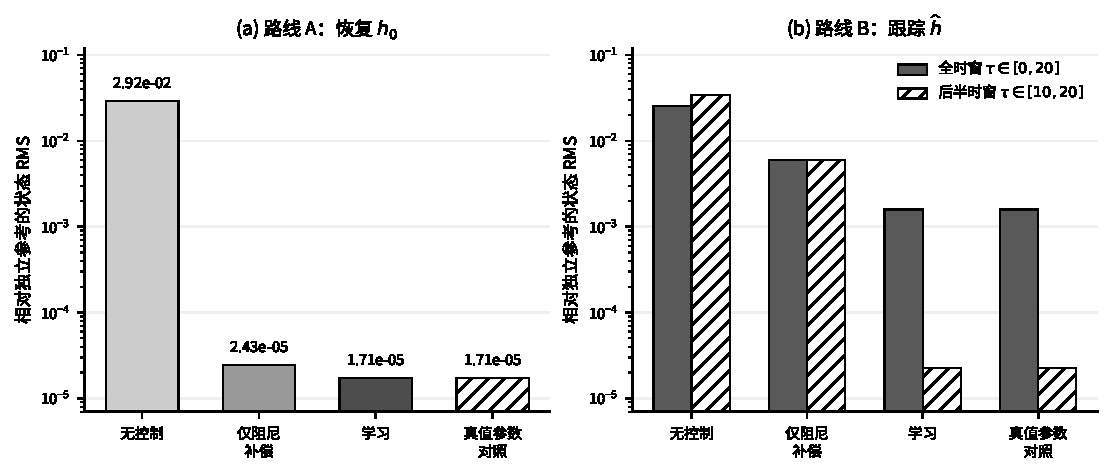
\includegraphics[width=\textwidth]{figures/new_baseline_results.pdf}
\caption{采用独立保守参考的新基准比较。
(a) 路线 A 从相同初态恢复 $h_0$。
(b) 路线 B 从非零初始偏差出发，跟踪冻结的 $\widehat h$ 轨迹。
全时窗与后半时窗误差揭示了跟踪暂态。
两个面板使用不同参考对象，因此柱高不能用于对两条路线作优劣排序。}
\label{num:results}
\end{figure*}

\subsection{路线 B 预测与跟踪协议}
\label{sx:route-b}
路线 B 脚本重新生成同一组训练与验证数据，
并检查其新拟合的系数向量与路线 A 向量的差异是否在 $10^{-13}$ 以内。
随后针对 $h_0$、$\widehat h$ 和 $h_*$ 分别计算三条保守轨迹，
采用 RK4 步长 $0.00025$，从共同初态积分至 $\tau=20$。
预测误差将 $h_0$ 和 $\widehat h$ 与 $h_*$ 比较；
后者是合成真值，而非独立物理数据。
对 $\widehat h$ 和 $h_*$ 参考，均另用 RK4 以步长 $0.0005$ 计算进行核查。

反馈控制的参考是冻结的保守 $\widehat h$ 流，
初态为 $(0.09,0.08,0.015,-0.01)$。
实际初态为 $(0.0945,0.084,0.015,-0.01)$。
位置偏差分别为参考各位置坐标的 $5\%$，动量偏差为零。
在无量纲时间下，增益取 $\kappa_p=1$、$\kappa_d=2$。
无控制、基于拟合参数的仅阻尼补偿、学习跟踪和真值参数对照跟踪组均使用同一参考。
学习指令与真值参数对照指令分别对应式~\eqref{struct:route-b-control} 和式~\eqref{struct:route-b-oracle} 中的不同控制律；
真值参数对照使用真实受控对象系数进行抵消，但保留拟合参考轨迹。

四个实际状态变量与四个参考变量共同构成八维中点求解，
Newton 设置与式~\eqref{sx:newton-stop} 相同。
独立 RK4 轨迹不输入该控制器，
仅在计算后用于报告式~\eqref{num:reference-split} 中的积分误差分量。
另一次计算将中点步长减半至 $0.0005$；
实际状态在共同时间点处的最大差值为 $2.22701\times10^{-5}$，
参考误差缩小 $3.999984$ 倍。
在记录的检查中，解析增广 Jacobian 与有限差分的最大差异为 $3.6902\times10^{-11}$。
这些有限差分是实现诊断，不能替代已经推导的 Jacobian。

对于真值参数对照，初始动量误差向量为零，连续误差满足
$e_X(\tau)=(1+\tau)e^{-\tau}e_X(0)$ 和
$e_Y(\tau)=-\tau e^{-\tau}\mathsf N^{-1}e_X(0)$。
还将离散误差与独立构造的该线性系统 Cayley 更新进行比较。
这一比较利用已知误差方程检验反馈与参考之间的耦合。

\subsection{跟踪敏感性与合并保留图表}
\label{xtr:shared-results}
五个阻尼设置使用与补充材料第~\ref{sx:damping}~节恢复实验相同的重新生成观测和重新拟合结果。跟踪实验持续 $\tau=10$，中点步长为 $0.002$，独立 RK4 步长为 $0.00025$；跟踪后半时窗为 $[5,10]$。这里对每个声明阻尼值独立拟合，并非让一个冻结控制器面对未知变化阻尼。下表保留两种目标，以明确显示它们不同的时间窗。

\begin{table*}[t]
\centering
\caption{阻尼扫描中相对于独立参考的状态均方根误差。
两条路线使用不同的目标哈密顿量与时间窗口。}
\label{sx:damping-errors}
\begin{tabular}{rcccc}
\toprule
$\zeta_1^{\mathrm{d}}$ & A 无控制，$[0,10]$ & A 学习，$[0,10]$ & B 无控制，$[5,10]$ & B 学习，$[5,10]$\\
\midrule
$0$ & $3.77362\times10^{-5}$ & $3.42885\times10^{-5}$ & $6.02444\times10^{-3}$ & $1.09567\times10^{-4}$ \\
$0.01$ & $6.73657\times10^{-3}$ & $3.42885\times10^{-5}$ & $3.71321\times10^{-3}$ & $1.09567\times10^{-4}$ \\
$0.025$ & $1.59501\times10^{-2}$ & $3.42885\times10^{-5}$ & $1.62063\times10^{-2}$ & $1.09567\times10^{-4}$ \\
$0.05$ & $2.92396\times10^{-2}$ & $3.42885\times10^{-5}$ & $3.42497\times10^{-2}$ & $1.09567\times10^{-4}$ \\
$0.1$ & $4.97374\times10^{-2}$ & $3.42885\times10^{-5}$ & $6.13727\times10^{-2}$ & $1.09567\times10^{-4}$ \\
\bottomrule
\end{tabular}
\end{table*}

\begin{figure*}[t]
\centering
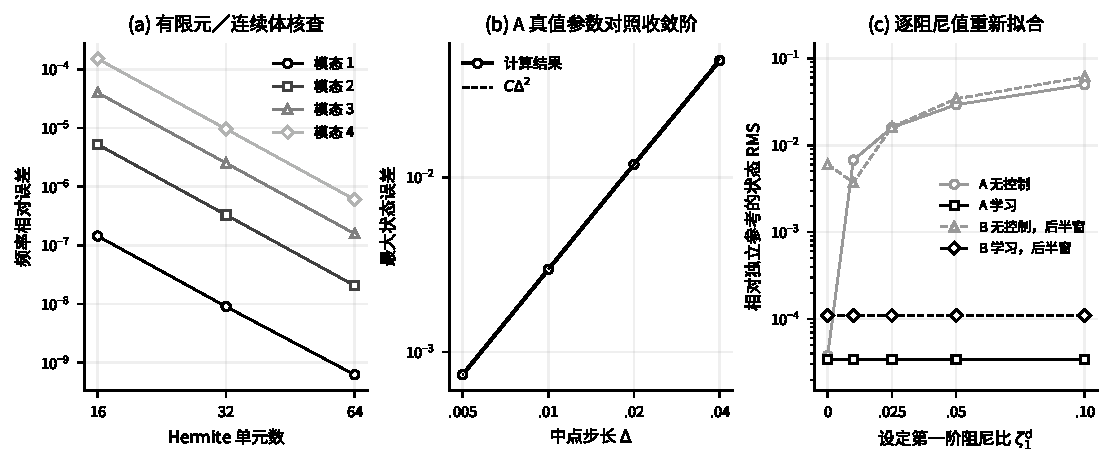
\includegraphics[width=\textwidth]{figures/new_baseline_verification.pdf}
\caption{根据随附 JSON 记录进行的独立数值核查。(a) 前四阶有限元频率收敛至连续体端点行列式的根。(b) 相对独立 RK4 参考，路线 A 真值参数对照误差以二阶收敛。(c) 每个阻尼设置均先重新拟合，再评价两条路线；A 使用完整 $[0,10]$ 时窗，B 使用后半 $[5,10]$ 时窗。连线仅连接已测试设置，不表示额外仿真或统计区间。}
\label{num:verification}
\end{figure*}
\begin{table*}[t]
\centering
\caption{补充学习跟踪实验中的采样局部磁需求。这是理想指令需求，并非硬件能力测量。}
\label{xtr:port-table}
\begin{tabular}{lcccc}
\toprule
实验 & $\max|B_y|$ (mT) & $\max|B|$ (mT) & $\max\|\nabla B\|_2$ (T/m) & $\max|F_y|$ ($\mu$N)\\
\midrule
B：学习 & $2.197941$ & $30.080408$ & $0.03453753$ & $0.611950$ \\
\bottomrule
\end{tabular}
\end{table*}

\clearpage
\begin{thebibliography}{99}

\bibitem[Abbott et~al.(2020)]{abbott}
Abbott JJ, Diller E and Petruska AJ (2020) Magnetic methods in robotics.
\textit{Annual Review of Control, Robotics, and Autonomous Systems} 3: 57--90.
\doi{10.1146/annurev-control-081219-082713}

\bibitem[Antman(2005)]{antman}
Antman SS (2005) \textit{Nonlinear Problems of Elasticity}. 2nd ed. Springer.
\doi{10.1007/0-387-27649-1}

\bibitem[Chen et~al.(2022)]{chen2022}
Chen Y, Matsubara T and Yaguchi T (2022) KAM theory meets statistical learning theory:
Hamiltonian neural networks with non-zero training loss.
\textit{Proceedings of the AAAI Conference on Artificial Intelligence} 36(6): 6322--6332.
\doi{10.1609/aaai.v36i6.20582}

\bibitem[Cho et~al.(2021)]{cho2021pdms}
Cho HS, Moon HY, Lee HS, Kim YT and Jeoung SC (2021) Formulation prediction for Young's modulus of poly(dimethylsiloxane) by spectroscopic methods.
\textit{Bulletin of the Korean Chemical Society} 42(9): 1225--1231. \doi{10.1002/bkcs.12352}

\bibitem[Desai et~al.(2021)]{desai}
Desai SA, Mattheakis M, Sondak D, Protopapas P and Roberts SJ (2021)
Port-Hamiltonian neural networks for learning explicit time-dependent dynamical systems.
\textit{Physical Review E} 104: 034312. \doi{10.1103/PhysRevE.104.034312}

\bibitem[Feng and Qin(2010)]{fengqin}
Feng K and Qin M (2010) \textit{Symplectic Geometric Algorithms for Hamiltonian Systems}. Springer.
\doi{10.1007/978-3-642-01777-3}

\bibitem[Feng et~al.(1989)]{feng}
Feng K, Wu HM, Qin MZ and Wang DL (1989) Construction of canonical difference
schemes for Hamiltonian formalism via generating functions.
\textit{Journal of Computational Mathematics} 7(1): 71--96.
\url{https://computmath.cjoe.ac.cn/jcm/EN/Y1989/V7/I1/71}.

\bibitem[Fischer et~al.(2017)]{fischer2017adhesion}
Fischer SCL, Kruttwig K, Bandmann V, Hensel R and Arzt E (2017) Adhesion and cellular compatibility of silicone-based skin adhesives.
\textit{Macromolecular Materials and Engineering} 302(5): 1600526. \doi{10.1002/mame.201600526}

\bibitem[Francescon et~al.(2025)]{francescon2025shape}
Francescon V, Murasovs N, Lloyd P, Onaizah O, Chathuranga DS and Valdastri P (2025)
Closed-loop shape-forming control of a magnetic soft continuum robot.
\textit{IEEE Robotics and Automation Letters} 10(6): 6071--6078.
\doi{10.1109/LRA.2025.3565124}

\bibitem[Greydanus et~al.(2019)]{greydanus}
Greydanus S, Dzamba M and Yosinski J (2019) Hamiltonian neural networks.
In: \textit{Advances in Neural Information Processing Systems}, vol. 32.
\url{https://arxiv.org/abs/1906.01563}.

\bibitem[Hairer et~al.(2006)]{hairer}
Hairer E, Lubich C and Wanner G (2006) \textit{Geometric Numerical Integration:
Structure-Preserving Algorithms for Ordinary Differential Equations}. 2nd ed. Springer.
\doi{10.1007/3-540-30666-8}

\bibitem[Haro and Luque(2019)]{haro2019aposteriori}
Haro \`A and Luque A (2019) A-posteriori KAM theory with optimal estimates for
partially integrable systems. \textit{Journal of Differential Equations}
266(2--3): 1605--1674. \doi{10.1016/j.jde.2018.08.003}
Preprint version used: \url{https://arxiv.org/abs/1711.05515v1}.

\bibitem[Hornik(1991)]{hornik}
Hornik K (1991) Approximation capabilities of multilayer feedforward networks.
\textit{Neural Networks} 4(2): 251--257. \doi{10.1016/0893-6080(91)90009-T}

\bibitem[Kim et~al.(2019)]{kim}
Kim Y, Parada GA, Liu S and Zhao X (2019) Ferromagnetic soft continuum robots.
\textit{Science Robotics} 4(33): eaax7329. \doi{10.1126/scirobotics.aax7329}

\bibitem[K\&J Magnetics(2026)]{kjMoment}
K\&J Magnetics (accessed 28 October 2026) Magnetic dipole moment.
\url{https://www.kjmagnetics.com/blog/magnetic-dipole-moment}.
Engineering dipole-moment approximation.

\bibitem[Lussi et~al.(2021)]{lussi2021cvs}
Lussi J et~al. (2021) A submillimeter continuous variable stiffness catheter for compliance control.
\textit{Advanced Science} 8(18): 2101290. \doi{10.1002/advs.202101290}

\bibitem[P\"oschel(2001)]{poschel}
P\"oschel J (2001) A lecture on the classical KAM theorem.
In: \textit{Proceedings of Symposia in Pure Mathematics}, vol. 69, pp. 707--732.
\doi{10.1090/pspum/069/1858551}
Preprint version used: \url{https://arxiv.org/abs/0908.2234v1} (Version 1.3, 2009).

\bibitem[Shang(1999)]{shang}
Shang ZJ (1999) KAM theorem of symplectic algorithms for Hamiltonian systems.
\textit{Numerische Mathematik} 83: 477--496. \doi{10.1007/s002110050460}

\bibitem[Simo(1985)]{simo}
Simo JC (1985) A finite strain beam formulation. The three-dimensional dynamic problem.
Part I. \textit{Computer Methods in Applied Mechanics and Engineering} 49(1): 55--70.
\doi{10.1016/0045-7825(85)90050-7}

\bibitem[SM Magnetics(2026)]{smN50}
SM Magnetics / SuperMagnetMan (accessed 28 October 2026) Magnet material grades: NdFeB stock grades, N50.
\url{https://supermagnetman.com/pages/magnet-material-grades}.
Manufacturer grade range, not an individual magnet calibration.

\bibitem[Su et~al.(2007)]{su2007}
Su HL, Sun YJ, Qin MZ and Scherer R (2007) Structure preserving schemes for Birkhoffian systems.
\textit{International Journal of Pure and Applied Mathematics} 40(3): 341--366.
\url{https://www.ijpam.eu/contents/2007-40-3/4/4.pdf}.

\bibitem[Tong et~al.(2025)]{tong2025navigation}
Tong D, Hao Z, Li J, Sun B, Liu M, Wang L and Huang W (2025)
Real-time simulation enabled navigation control of magnetic soft continuum robots in confined lumens.
\textit{Journal of the Mechanics and Physics of Solids} 203: 106198.
\doi{10.1016/j.jmps.2025.106198}

\bibitem[Trabelsi et~al.(2018)]{trabelsi}
Trabelsi C, Bilaniuk O, Zhang Y et~al. (2018) Deep complex networks.
In: \textit{International Conference on Learning Representations}.
\url{https://arxiv.org/abs/1705.09792}.

\bibitem[Zhang et~al.(2022)]{zhang}
Zhang SQ, Gao W and Zhou ZH (2022) Towards understanding theoretical advantages of
complex-reaction networks. \textit{Neural Networks} 151: 80--93.
\doi{10.1016/j.neunet.2022.03.024}
\href{https://www.lamda.nju.edu.cn/zhangsq/papers/2022-CRNet-NN.pdf}{Published version used for theorem numbering}.

\bibitem[Zhong et~al.(2020)]{zhong}
Zhong YD, Dey B and Chakraborty A (2020) Dissipative SymODEN: Encoding Hamiltonian
dynamics with dissipation and control into deep learning.
In: \textit{ICLR Workshop on Integration of Deep Neural Models and Differential Equations}.
\url{https://arxiv.org/abs/2002.08860}.
\end{thebibliography}

\end{document}
